\SourcePage{GELFAND-P000034}{unlabelled}
\underline{What do we know?} Char. of the gr. of real matr. with $\det=1$.
\uwave{Complex} ---
\par\noindent\begin{minipage}{\linewidth}
\begin{equation*}
\sigma(g)=\frac{\pi(\lambda_{\textcolor{orange!65!black}{g}})+\pi(\lambda_g^{-1})}{|\lambda_g-\lambda_g^{-1}|^2}.
\end{equation*}
\Unclear{GELFAND-P000034}{complex-first-subscript}{The lower stroke by the first $\lambda$ in the numerator merges into the right parenthesis. The subscript $g$ is provisional.}
\end{minipage}\par
[At right: Gelfand, Naimark, 1947.]
$\pi(\lambda_g)$ --- a mult. character of the field of complex numbers.
\underline{Real.}
\begin{equation*}
\sigma(g)=\begin{cases}
\dfrac{\pi(\lambda_g)+\pi(\lambda_g^{-1})}{|\lambda-\lambda^{-1}|}&\text{if }\lambda\text{ is real.},\\
0&\text{if }\lambda\text{ is complex.}
\end{cases}
\end{equation*}
\begin{equation*}
\sigma'(g)=\begin{cases}
\dfrac{\pi(\lambda_{\min})}{|\lambda-\lambda^{-1}|}&\text{if }\lambda\text{ is real.},\\
\dfrac{\pi(\lambda_g)+\pi(\lambda_g^{-1})}{|\lambda-\lambda^{-1}|}
-\dfrac{\pi(\lambda_g)-\pi(\lambda_g^{-1})}{\lambda_g-\lambda_g^{-1}}&
\end{cases}
\end{equation*}
[No condition is written at right in the second row of the last brace. In the left margin, rotated:]
\textcolor{orange!65!black}{Vanguten / Vantsuten}, 1947.
\Unclear{GELFAND-P000034}{real-margin-name}{The marginal surname resembles Вангутен / Ванцутен [Vanguten / Vantsuten]. Its joined middle strokes remain uncertain; the written year is 1947.}
\par\noindent\begin{minipage}{\linewidth}
[Cancelled; provisional reading: \textcolor{orange!65!black}{repr. [предст.; uncertain reading]}]
\Unclear{GELFAND-P000034}{padic-cancellation}{The crossed-out source abbreviation resembles предст. [repr.]; a horizontal cancellation and two long strokes below it obscure parts of the letters.}
\end{minipage}\par
\par\noindent\begin{minipage}{\linewidth}
\underline{$p$-adic numbers.}
\begin{equation*}
\sigma(g)=\begin{cases}
\dfrac{\pi(\lambda_g)+\pi(\lambda_g^{-1})}{|\lambda_g-\lambda_g^{-1}|}&\text{if }\lambda_g\in K\text{ is real.},\\
0&\lambda_g{\overline{\in}}K.
\end{cases}
\end{equation*}
[Nonmembership is written in the source with a bar over $\in$. At right, beside a long vertical stroke:]
\begin{tabular}{|l}Gelfand,\\Graev,\\1963.\end{tabular}
\end{minipage}\par\medskip
\underline{Finite field.}
\begin{equation*}
\sigma(g)=\begin{cases}
\pi(\lambda_g)+\pi(\lambda_g^{-1})&\lambda\in K,\\
0&\lambda{\overline{\in}}K,
\end{cases}
\end{equation*}
[At right: Frobenius, 1895.]
\begin{equation*}
\sigma'(g)=\begin{cases}
0&\lambda\in K,\\
-\pi(\lambda_g)-\pi(\lambda_g^{-1})&\lambda{\overline{\in}}K.
\end{cases}
\end{equation*}

\Needspace{5\baselineskip}
\SourcePage{GELFAND-P000035}{18}
\par\noindent\begin{minipage}{\linewidth}
\textcolor{orange!65!black}{Nat. res. [рез.; provisional] [сост.; abbreviated]} was that one must pass to the group of \uwave{adeles}.
\Unclear{GELFAND-P000035}{top-abbreviations}{The first and third source abbreviations read Ест. and сост. The middle is provisionally read as рез. [res.]; the middle strokes are joined.}
\end{minipage}\par
\underline{Gr. of adeles} --- the direct $\sum$ of the gr. of all $p$-adic numbers.
In it there are rational numbers --- the \uwave{diagonal}.

\underline{Vishik.}
\SourceFigure{GELFAND-P000035}{vishik-strip}{Beneath the surname is a narrow strip with irregular long edges and transverse strokes. Two strokes near the left meet at the lower edge; the following dividers have unequal spacing. No labels are written inside.\par\smallskip\centering\resizebox{.98\linewidth}{!}{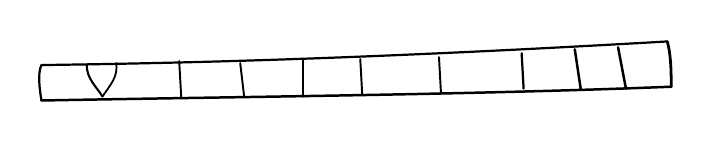
\begin{tikzpicture}[x=.025cm,y=-.025cm,line cap=round,line join=round]
\path[use as bounding box](10,5)rectangle(345,50);
\draw[line width=.8pt](17,24)..controls(88,23)and(179,21)..(335,12);
\draw[line width=.9pt](17,42)..controls(125,40)and(237,39)..(337,35);
\draw[line width=.8pt](17,24)..controls(15,28)and(16,36)..(17,42);
\draw[line width=1pt](335,12)..controls(337,19)and(337,29)..(337,35);
\draw[line width=.75pt](40,24)..controls(40,31)and(45,35)..(48,40);
\draw[line width=.65pt](55,23)..controls(56,30)and(52,34)..(48,40);
\draw[line width=.7pt](87,22)--(88,40);
\draw[line width=.7pt](118,23)--(120,40);
\draw[line width=.7pt](150,21)--(150,40);
\draw[line width=.7pt](179,21)--(180,39);
\draw[line width=.7pt](219,20)--(220,38);
\draw[line width=.8pt](261,18)--(262,36);
\draw[line width=.9pt](288,16)--(291,36);
\draw[line width=.9pt](310,15)--(314,36);
\end{tikzpicture}}}
What one should work on in diff. eqns.
For a lin. oper. with finite kernel and cokernel an index is introduced.
\begin{equation*}
k=\dim\ker T,\qquad
\ell=\dim\operatorname{coker}K,\qquad
\text{æ}=k-\ell.
\end{equation*}
\Unclear{GELFAND-P000035}{index-definition}{The letter after coker resembles $K$. The looped index sign is represented by the provisional candidate æ; its exact letter has not been established.}
1) If replaced by $\|T-T_1\|<\varepsilon$, then æ does not change.
2) Adding a \textcolor{orange!65!black}{compl. cont. [вп. непр.; abbreviated reading]} oper. does not change the index.
\Unclear{GELFAND-P000035}{compact-operator}{The source writes Доб. вп. непр. опер. [Adding a compl. cont. oper.]. The joined abbreviations are shown in their written form; the full words are not written out.}
æ allows classification of elliptic eqns. on manifolds.
(Atiyah and Singer) Homotopy classification.
Vishik considers that the index is the only homotopy inv.
\par\noindent\begin{minipage}{\linewidth}
A syst. with const. coeffs. in a ball has [a short entry is cancelled]
as one more homot. inv.
[Beneath this is a long cancelled parenthetical entry.]
\Unclear{GELFAND-P000035}{middle-cancellations}{A short entry after имеет [has] is cancelled; its descending loop remains visible. Beneath it a long parenthetical entry is crossed out with two horizontal lines; its ending resembles инв. [inv.]. The text remains unreadable.}
\end{minipage}\par
Can any one be transformed into any other
(a large number of eqns. --- stable).
The question has an analogous meaning for a different class of nonlinear eqns. What is æ?
What are the kernel and cokernel?
$\sim$ a finite kernel.
Quasilin. eqn.
\begin{equation*}
Tu=v.
\end{equation*}
[At right: $u$ --- a manifold. It is required to be finite dimensional.]
Principal part of a nonlinear eqn.
\underline{Cokernel} $\sim$ [a short wavy line].
[At right: In each point, linearize the eqn., and everywhere it is the same.]
\uwave{Problem}: study the index of a nonlinear elliptic eqn.
(This is an integral question.)
Quasilin.
\begin{equation*}
\sum A(\ldots u_0)\frac{\partial^2u}{\partial x^2}.
\end{equation*}
\Unclear{GELFAND-P000035}{nonlinear-formula}{The lower sign on $u$ in the argument of $A$ resembles $0$ / $\omega$; the joined dark strokes do not establish which. The dots and absence of sum indices are retained.}

\par\noindent\begin{minipage}{\linewidth}
\underline{\textcolor{orange!65!black}{16th.}} Linnik --- “\uwave{How to use funct. anal. in probability theory}”.
\Unclear{GELFAND-P000035}{linnik-date}{The small marks after 16 are provisionally read as the Russian ordinal suffix го. They could also be digits.}
\end{minipage}\par

\Needspace{5\baselineskip}
\par\noindent\begin{minipage}{\linewidth}
\SourcePage{GELFAND-P000036}{unlabelled}
\textcolor{orange!65!black}{I. I. / I. M.}\ Pyatetsky-Shapiro.
\Unclear{GELFAND-P000036}{speaker-initials}{I. I. / I. M. Pyatetsky-Shapiro. The second initial is merged; its exact reading is not established.}
\end{minipage}\par
(Ilya Iosifovich). \uwave{Linnik's work.}
\begin{equation*}
x^2+y^2+z^2=m.
\end{equation*}
\par\noindent\begin{minipage}{\linewidth}
[At left:] \textcolor{orange!65!black}{$\phi$}.
\Unclear{GELFAND-P000036}{left-sign}{A separate looped sign with a right vertical stroke in the left margin resembles $\phi$. No meaning is written beside it.}
\end{minipage}\par
For which $m$ are there integral solutions?
It is known that solutions do not always exist.
(When $m=8a+7$, there are no solutions.) [Beneath $8a+7$: mod 8.]
How the solutions are distributed on the surface of the 3-dimensional sphere.
Rad. $m^{1/2}$.
\SourceFigure{GELFAND-P000036}{sphere-projection}{Two irregular rounded contours, labels $1$ and $\sqrt m$, diverging lines, three heavy points and a thick inner junction with a small leftward arrow. The junction of the inner strokes is not wholly clear.\par\smallskip\centering\color{black}\begin{tikzpicture}[x=.19mm,y=-.19mm,line width=.55pt]
\path[use as bounding box] (0,0) rectangle (325,260);
\draw (115,12) .. controls (162,4) and (204,38) .. (207,70) .. controls (228,125) and (183,187) .. (108,198) .. controls (35,206) and (0,137) .. (18,100) .. controls (19,55) and (65,12) .. (115,12);
\draw (113,78) .. controls (137,73) and (153,79) .. (153,94) .. controls (164,116) and (131,136) .. (107,130) .. controls (85,124) and (86,98) .. (90,90) .. controls (95,81) and (104,78) .. (113,78);
\draw (115,100) -- (145,87) -- (204,70);
\draw (115,100) .. controls (130,110) and (137,117) .. (152,117) -- (202,126);
\draw[line width=1pt] (112,98) -- (124,102) -- (131,99);
\draw (132,98) -- (123,102) -- (130,109);
\fill (115,100) circle (2);\fill (145,87) circle (2.8);\fill (204,70) circle (3);\fill (202,126) circle (3);
\node at (110,48) {$1$};\node at (255,137) {$\sqrt m$};
\end{tikzpicture}}
Select a region on the unit sphere and see how many points project into it.
\par\noindent\begin{minipage}{\linewidth}
\begin{equation*}
\frac{H_2(m)}{H(m)}\approx\operatorname{mes}\Omega.
\end{equation*}
\Unclear{GELFAND-P000036}{class-number-annotation}{The numerator subscript resembles $2$; $\Omega$ remains an alternative. Beneath $H(m)$: total number. At right: \uwave{nat. hypothesis}; below: but there are $m$ for which few. The last abbreviated entry is not wholly clear.}
\end{minipage}\par
\par\noindent\begin{minipage}{\linewidth}
This holds under the following condition:
if $q$ is a prime
\underline{$m$ \textcolor{orange!65!black}{ranges over / пробл. [пробег. / пробл.; uncertain abbreviation]}\ numbers:} $\xi^2+m=0\ (\operatorname{mod}q)$ is solvable.
\Unclear{GELFAND-P000036}{q-condition}{Underlined: $m$ пробег. / пробл. числа [$m$ ranges over / пробл. numbers; uncertain abbreviated readings]. The middle and final strokes are joined; the second candidate is not expanded.}
\end{minipage}\par
For \textcolor{orange!65!black}{any / small [любой / небол.; uncertain readings]}\ such seq. this theorem holds.
\Unclear{GELFAND-P000036}{sequence-line}{The joined word after For resembles любой [any]; it is followed by такой послед. [such seq.]. небол. [small; abbreviated reading] remains an alternative for the dark initial strokes.}
Using $q$, construct a dyn. system on the sphere,
whose behaviour obeys prob. laws:
Fix $q$, consider [a short entry is cancelled] an integral point on the sphere and all orthog. matrices with entries of the form $a/q$.
\Unclear{GELFAND-P000036}{dynamics-cancellation}{Before integral point, a short entry is cancelled with several dense strokes; the text has not been read.}
($a$ is an integer.) There are finitely many of them, but many.
They carry an integral point to a non-integral one.
But among them there are finitely many carrying an integral point to an integral one.
Construct such a flow
(each point its own $48$ orthog. matrices).
$e$ is a characteristic fn.
\begin{equation*}
e(Tx)+e(T^2x).
\end{equation*}
[Rightward arrow: \uwave{to the area}.]
This is a Markov chain.

\Needspace{5\baselineskip}
\par\noindent\begin{minipage}{\linewidth}
\SourcePage{GELFAND-P000037}{19}
\underline{Povzner.} \underline{Naum Yakovlevich.}
\uwave{Plan of stat. physics.} \uwave{Int. works.}
\begin{equation*}
\begin{array}{ll}\text{Ruelle}&\text{2--3 works}\\\text{Yang Lee}&\text{1 work}\end{array}
\end{equation*}
\SourceFigure{GELFAND-P000037}{statistical-work-bracket}{The line steps down beside the list of works; its right segment runs beneath “Yang Lee”.\par\smallskip\centering\begin{tikzpicture}[x=1mm,y=1mm,line width=.65pt]\draw (0,4)--(20,4)--(20,0)--(48,0);\end{tikzpicture}}
\end{minipage}\par
This is a revolution. Everything known mathematically about stat. physics.
Kac --- \uwave{models}.
\underline{Problem.} (Elem.)
\SourceFigure{GELFAND-P000037}{pair-potential}{A vertical with $u$, a horizontal with $0$ at right; the curve falls steeply below the horizontal and then rises towards it at right. The right part is thickened. At left: grows. The precise junction of the thick strokes is not wholly clear.\par\smallskip\centering\color{black}\begin{tikzpicture}[x=.15mm,y=-.15mm,line width=.6pt]
\path[use as bounding box] (0,20) rectangle (465,250);
\draw (175,50) -- (181,210);
\draw (117,133) .. controls (175,142) and (310,129) .. (414,123);
\draw (191,50) .. controls (193,97) and (195,163) .. (203,183) .. controls (208,209) and (226,196) .. (250,168) .. controls (275,150) and (322,143) .. (370,135);
\draw[line width=1.7pt] (300,150) -- (333,142) -- (360,136);
\node at (159,41) {$u$};\node at (387,103) {$0$};\node at (70,75) {grows};
\end{tikzpicture}}
\begin{equation*}
\min\sum_{i,j=1}^{N}u(x_i-x_j).
\end{equation*}
\SourceFigure{GELFAND-P000037}{configuration-bracket}{The line beneath the sum steps upward toward the note at right.\par\smallskip\centering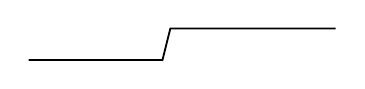
\begin{tikzpicture}[x=1mm,y=1mm,line width=.65pt]\draw (0,0)--(17,0)--(18,4)--(39,4);\end{tikzpicture}}
$x$ ranges in 2-dimensional space.\par
\underline{Set of $x$.}
There is a $C$ such that the min. config. has everything in a sphere of rad. $C$.
(Easy to show $N^2$, but in the case of a sphere $N^3$.)
[Separate thick lines beneath $N^2$ and case.]

16/\underline{$\overline{\mathrm{XI}}$}
\underline{A lin. operator in Hilbert space has an inv. subspace.}
Solved!!!
Bull. Amer. Math. Soc.
\par\noindent\begin{minipage}{\linewidth}
\uwave{\textcolor{orange!65!black}{Lui de Brange}} and \ldots
\Unclear{GELFAND-P000037}{de-brange-name}{The entry reads Lui de Brange and ...; the surname ending is looped, with a possible final s. Year: 1964.}
\end{minipage}\par
1964.
Connected with Livshits's theory.
\par\noindent\begin{minipage}{\linewidth}
[Below at left:] \textcolor{orange!65!black}{$\phi$ / $\psi$}.
\Unclear{GELFAND-P000037}{left-sign}{A separate sign in the left margin has two upper strokes and a right lower loop; graphic candidates are $\phi$ / $\psi$. There is no caption.}
\end{minipage}\par
\underline{det} by Schur.
One must take the substitution group, and instead of all --- \underline{repr.}
$\det$ of a + definite matrix is a + definite matrix.

\underline{Arnold.}
Consider a dyn. system and the corresponding quantum system.
\SourceFigure{GELFAND-P000037}{quantum-packet}{A nearly round contour around the intersection of a vertical and a horizontal rightward arrow labelled $x$. Inside are irregular vertical and wavy strokes; some intersections merge.\par\smallskip\centering\color{black}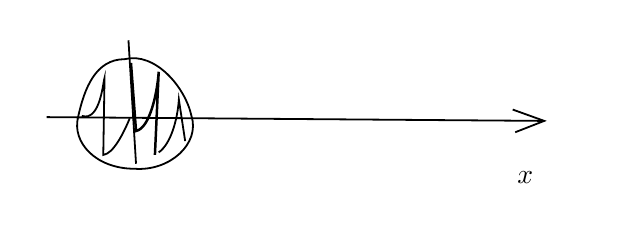
\begin{tikzpicture}[x=.16mm,y=-.16mm,line width=.65pt]
\path[use as bounding box] (0,30) rectangle (450,180);
\draw (15,101) -- (410,104);\draw (385,95) -- (410,104) -- (387,113);
\draw (80,40) -- (86,138);
\draw (77,55) .. controls (101,49) and (125,77) .. (130,100) .. controls (137,122) and (113,144) .. (85,142) .. controls (54,142) and (35,121) .. (40,101) .. controls (45,78) and (54,55) .. (77,55);
\draw (43,100) .. controls (58,105) and (60,71) .. (61,70) -- (60,131) .. controls (68,130) and (76,114) .. (81,102);
\draw[line width=.9pt] (82,58) -- (86,112) .. controls (97,110) and (103,81) .. (104,65) -- (101,131);
\draw (104,129) .. controls (114,122) and (119,102) .. (120,87) -- (125,120);
\node at (395,149) {$x$};
\end{tikzpicture}}
\begin{equation*}
\psi(x)e^{\frac{i}{h}S(x)}.
\end{equation*}
Quantum particle.
\begin{equation*}
\psi\in\mathcal D(\mathbf R^n),\qquad S(x)=\int p\,dx.
\end{equation*}
$h$ is Planck's const.
Seek the solution in the same form.
A semiclass. asymptotic is obtained.
\SourceFigure{GELFAND-P000037}{bottom-trajectory}{Unlabelled axes. A heavy point lies at right above the horizontal; an arch goes up and right from it, then down to a right arrowhead. No continuation beyond the frame is shown.\par\smallskip\centering\color{black}\begin{tikzpicture}[x=.15mm,y=-.15mm,line width=.65pt]
\path[use as bounding box] (0,0) rectangle (455,195);
\draw (127,10) -- (118,160);\draw (29,140) .. controls (135,153) and (328,144) .. (431,157);
\fill (199,76) ellipse (7 and 10);
\draw (199,76) .. controls (229,43) and (281,35) .. (316,39) .. controls (356,39) and (375,62) .. (387,76);
\draw (378,54) -- (391,76) -- (365,79);
\end{tikzpicture}}

\Needspace{5\baselineskip}
\par\noindent\begin{minipage}{\linewidth}
\SourcePage{GELFAND-P000038}{unlabelled}
\begin{equation*}
\frac{\psi(\xi(x))e^{\frac{i}{h}(S(x)+\int p\,dx)}}{\sqrt{\dfrac{D(X)}{D(x)}}}.
\end{equation*}
\Unclear{GELFAND-P000038}{semiclassical-amplitude}{The argument of $\psi$ is overwritten: $\xi(x)$ / $x$. The sign after $S(x)$ resembles $+$ / $t$. Under the radical the upper argument letter resembles $X$ / $x$; no separate index is visible.}
\end{minipage}\par
[At right: norm. factor.]
Holds only as $h\longrightarrow0$, but when $D\ne0$.
(Through $t$, map. $D$ is the $\det$ of the new pts. in terms of the old ones.)
The solution of the question reduces to top. inv. of a manifold.
(At a turning point.) \underline{Index.}
[At right: During mov. one obtains a cohomology class.]

\underline{Linnik.}
\underline{Ideals of rings of fns. from the point of view of appl. to statistics.}
A. Cartan --- on ideals of rings of holom. fns. (47 and 50).
Analyt. sheaves appear (first with \uwave{Oka}).
Appl. of the apparatus of analyt. sheaves.
What is statistics?
\begin{equation*}
(X,A,\mu)\overset{T}{\longrightarrow}(Y,B).
\end{equation*}
[Beneath the first parentheses: space with measure. Beneath the second: space with a $\sigma$-system.]
$T$ is a measurable mapping (observation fn.).
$X$ is what we observe.
The measure on $Y$ is directly induced [a short entry is cancelled] from $X$.
\Unclear{GELFAND-P000038}{induced-measure-cancellation}{Between directly induced and from $X$, a short entry is heavily crossed out; the exact text is not established.}
$X$ is Euclidean space.
$A$ --- Borel sets.
\par\noindent\begin{minipage}{\linewidth}
$\mu$ --- measure.
(\textcolor{orange!65!black}{об. [abbrev.] set of measures, major. [мажор.; provisional] 1st}).
\Unclear{GELFAND-P000038}{measure-parenthesis}{In parentheses: об. набор. мер, мажор. / массы 1-й / 1-ой [об.; set of measures; major. / mass; 1st, uncertain abbreviated readings]. The joined strokes before 1-й are closer to мажор.; the exact abbreviation and ending remain uncertain.}
\end{minipage}\par
\par\noindent\begin{minipage}{\linewidth}
There is a family of measures $\left\{P(x,\theta)\right)$.
\EvidenceBlock{GELFAND-P000038}{family-delimiter}{After $P(x,\theta)$ a second round parenthesis is written.}{Manuscript notation.}
\end{minipage}\par
[Beneath $P(x,\theta)$: given by a density.]
We want to obtain info. about the parameter by observing $X$.
\begin{equation*}
x_1,\ldots,x_n\in N(a,1).
\end{equation*}
[Beneath $N(a,1)$: Gaussian family. At right: 1 is precision, $a$ is the parameter.]
\begin{equation*}
x_i=a+\Delta_i,\qquad\overline X\ \text{arithm. mean}
\end{equation*}
$\Delta_i$ --- normal.

\Needspace{5\baselineskip}
\SourcePage{GELFAND-P000039}{20}
\underline{Stat.} --- finding estimates.
Testing hypotheses $a=a_0$.
$\theta\in\Omega$.
($\Omega$ --- a comp. region in $\mathbf R^n$.)
Null hypothesis $H_0=\theta\in\omega$ (subspace).
\uwave{Testing with a fixed sample with randomization.}
A selected test is a fn. of the observations
\begin{equation*}
0\le\varphi(x_1,\ldots,x_n)\le1.
\end{equation*}
[Beneath the formula: prob. meaning.]
Observe with a random fn. and randomize with probabilities $\varphi$, $1-\varphi$.
[Cancellation at left and a separate sign below.]
\Unclear{GELFAND-P000039}{test-cancellation}{A short entry is heavily cancelled. Beneath it is a separate sign resembling $\pi$ / $\Pi$; no meaning is written.}
\par\noindent\begin{minipage}{\linewidth}
Simple test
\begin{equation*}
\varphi=\begin{cases}0\\1\end{cases}\qquad\begin{gathered}\text{reject}\\\text{or accept}\end{gathered}
\end{equation*}
\EvidenceBlock{GELFAND-P000039}{simple-test-labels}{Two short entries stand at right of $0$ and $1$. There are no visible lines connecting the entries to the values.}{Manuscript notation.}
\end{minipage}\par
[Downward arrow to the example:]
\begin{equation*}
|\overline x-a_0|>\varepsilon\qquad\text{reject or accept}
\end{equation*}
\uwave{Test quality is assessed as follows.}
\begin{equation*}
E(\varphi\mid H_0).
\end{equation*}
Expectation under hypothesis $H_0$ (param. $\in\omega$).
[At right: meaningful only if 1 point.]
$H_1$ --- alternative.
\par\noindent\begin{minipage}{\linewidth}
$\bigl(\overset{\theta}{H_1}\ \textcolor{orange!65!black}{\subset}\ \text{compl. }\omega\bigr)$.
\Unclear{GELFAND-P000039}{alternative-condition}{A separate $\theta$ stands over $H_1$. The following C-like sign may be $\subset$; it is followed by compl. $\omega$.}
\end{minipage}\par
\par\noindent\begin{minipage}{\linewidth}
\begin{equation*}
E(\varphi,H_a')\le\alpha,\qquad E(\varphi\mid H_1')=\max.
\end{equation*}
\Unclear{GELFAND-P000039}{null-expectation-subscript}{At left the lower sign at $H$ resembles $a$ / $0$, and the upper stroke resembles $\prime$ / $1$. There is a comma between $\varphi$ and $H$. At right the upper stroke at $H_1$ is separately visible.}
\end{minipage}\par
[Beneath the left expectation: simple hypothesis (fixed point). Beneath the right: (desirable).]
Reject the true one not too often, but also reject
[a short entry is cancelled] the false one often.
\Unclear{GELFAND-P000039}{lower-test-cancellation}{Before false, a tiny sign is heavily crossed out; the text beneath the cancellation has not been read.}
\uwave{Similar tests.}
(At each point of the null hypothesis the prob. is $\alpha$.)
\par\noindent\begin{minipage}{\linewidth}
\underline{Two examples.}
\SourceFigure{GELFAND-P000039}{gaussian-example-bracket}{A stepped lower line and a tall right edge surround the entry about the Gaussian sample.\par\smallskip\centering\resizebox{.98\linewidth}{!}{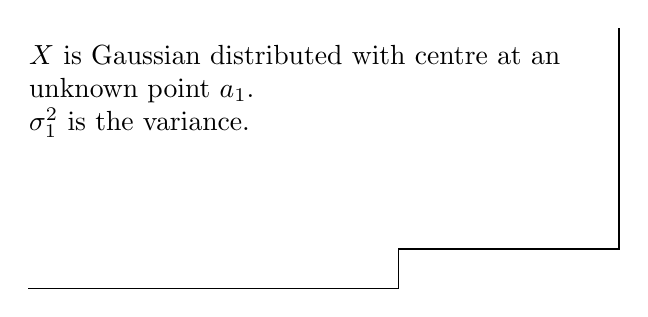
\begin{tikzpicture}[x=1mm,y=1mm,line width=.5pt]\node[anchor=north west,inner sep=0pt,text width=70mm] at (0,31) {$X$ is Gaussian distributed with centre at an unknown point $a_1$.\par $\sigma_1^2$ is the variance.};\draw (0,0)--(47,0)--(47,5)--(75,5)--(75,33);\end{tikzpicture}}}
\end{minipage}\par
Testing by means of inv. tests.
\Unclear{GELFAND-P000039}{invariant-test-cancellation}{In the continuation: null, below it a short cancellation and гип. / ил. The joined strokes after the cancellation do not give an exact reading.}
\par\noindent\begin{minipage}{\linewidth}
$\theta$ --- \textcolor{orange!65!black}{mult. [мног.; provisional]}\ $a_i$.
\Unclear{GELFAND-P000039}{theta-word}{$\theta$ --- мног. / мнот. $a_i$. The final stroke of the abbreviation resembles г / т; the reading is not established.}
\end{minipage}\par
\underline{Question.} $a_1=a_2$?
\begin{equation*}
N(a_1,\sigma_1^2),\qquad x_1,x_2,\ldots,x_n,
\end{equation*}
\begin{equation*}
N(a_2,\sigma_2^2),\qquad y_1,\ldots,y_n.
\end{equation*}
[At right: $\sigma_i^2$ are unknown param.]
\begin{equation*}
H_0:\quad a_1=a_2,
\end{equation*}
\begin{equation*}
E(\varphi\mid H_0')=\alpha,\qquad E(\varphi\mid H_1)=\max.
\end{equation*}
$\varphi$ --- ?

\Needspace{5\baselineskip}
\SourcePage{GELFAND-P000040}{unlabelled}
$\varphi$ is inv. or similar if for every $\theta$ the expectation of $\varphi$ is the same.
(For every $\theta$ there is a prob. distrib.)
\par\noindent\begin{minipage}{\linewidth}
\begin{equation*}
E(\varphi\mid H_0)=\alpha,\qquad E(\varphi\mid H_1')=\max.
\end{equation*}
[At right: \textcolor{orange!65!black}{[mark]}].
\Unclear{GELFAND-P000040}{right-hand-mark}{There is a separate dark mark to the right of the expectations. Its reading is uncertain.}
\end{minipage}\par
$H_1'$ is one point in the complement.
Bayesian measure is a measure on parameter space.
(Given beforehand --- a priori distribution.)
[At left a rightward arrow to the lines:]
The measure depends on a 4-tuple of points $(a_1,a_2,\sigma_1,\sigma_2)$.
\underline{Null hypothesis.}
\SourceFigure{GELFAND-P000040}{null-strip}{Beneath null hypothesis is an irregular narrow strip with diagonal strokes; $a_1$ and a comma stand separately at right. The right strokes merge with the upper edge.\par\smallskip\centering\color{black}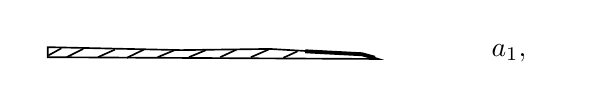
\begin{tikzpicture}[x=.075mm,y=-.075mm,line width=.6pt]
\path[use as bounding box] (0,30) rectangle (925,115);
\draw (34,63) -- (260,68) -- (410,66) -- (568,75) -- (594,83) -- (34,80) -- cycle;
\draw (35,77) -- (57,65) (66,80) -- (94,66) (119,80) -- (148,67) (168,81) -- (197,67) (220,80) -- (249,68) (273,80) -- (302,68) (326,80) -- (354,67) (378,80) -- (408,67) (433,81) -- (457,70);
\draw[line width=1.4pt] (470,70) -- (566,75) -- (588,81);
\node at (815,73) {$a_1,$};
\end{tikzpicture}}
\uwave{Bayes measure.}
\SourceFigure{GELFAND-P000040}{bayes-rectangle}{Beside Bayes measure is an empty rectangle: its thick top extends rightwards, and the lower line continues beyond both vertical sides. There is no label inside.\par\smallskip\centering\color{black}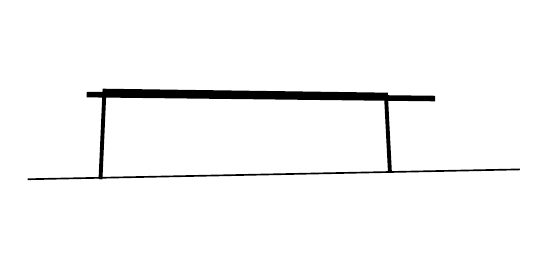
\begin{tikzpicture}[x=.25mm,y=-.25mm,line width=.6pt]
\path[use as bounding box] (0,0) rectangle (250,110);
\draw (0,77) -- (250,72);\draw[line width=1.4pt] (37,77) -- (39,32) -- (182,34) -- (184,73);
\draw[line width=2pt] (30,34) -- (207,36);
\end{tikzpicture}}
[At right: Unif. distrib., \textcolor{orange!65!black}{from [от.; provisional]}\ $0$.]
\Unclear{GELFAND-P000040}{radon-measure-tail}{The short entry before $0$ is provisionally read as от. [from].}
One must be able to solve for every Bayesian distrib.-measure.
\underline{Result:} A prob. distrib. in $X\times Y$ with a given Gaussian measure (4-param.).
Find $\varphi(x,y)$ such that
\par\noindent\begin{minipage}{\linewidth}
\begin{equation*}
E\bigl(\varphi(x_1,\ldots,x_{\textcolor{orange!65!black}{n}},y_1,\ldots,y_m)\bigr).
\end{equation*}
\Unclear{GELFAND-P000040}{sample-index}{The final subscript on $x$ resembles $n$ or $m$ and has two joined strokes. The subscript $m$ on $y$ is retained.}
\Unclear{GELFAND-P000040}{gaussian-condition}{At right: for every admiss. Gaussian measure ($=\alpha$ when $a_1=a_2$ and $\max$ integr. / param. [проинтегр. / параметр.; uncertain abbreviated readings] on the complement). The word after $\max$ is graphically closer to проинтегр.; neither candidate is asserted as certain.}
\end{minipage}\par
\underline{Sufficient statistic} --- contains all info. about the parameters.

\underline{Problem not done.}
$\theta_1$, $\theta_2$ are complex variables.
$f(\theta_1,\theta_2)$ in a ball, \uwave{ideals} are not known
(All prim. ideals corresponding to the ideal equal to 0.)
Glisson [Глиссон] --- ball and \uuline{centre} holom.
\par\noindent\begin{minipage}{\linewidth}
Suff. spec. ideals of fns., van. at $0$ on a \textcolor{orange!65!black}{$\theta$-th}\ fin. number of polynomials.
\Unclear{GELFAND-P000040}{terminal-ideals}{The first sign after the source word на is provisionally read as $\theta$; it may be $0$.}
\end{minipage}\par

\Needspace{5\baselineskip}
\SourcePage{GELFAND-P000041}{21}
Gleason — \underline{Gorin.}

\par\noindent\begin{minipage}{\linewidth}
J. Math. Mech. v.~13. N~1 (1964).
\Unclear{GELFAND-P000041}{volume}{The number $13$ is written over earlier strokes. The underlying numeral is uncertain.}
\end{minipage}\par

Consider a ball $z=(z_1,z_2)$,
\begin{equation*}
|z_1|^2+|z_2|^2\leq1
\end{equation*}
and fns., an. inside and cont. on the bdry., with $f(0,0)=0$.
Do there exist $g_1,g_2$ of the same type such that
\begin{equation*}
f=z_1g_1+z_2g_2
\end{equation*}
(max ideal; will $z_1,z_2$ be a basis?
This can be done inside, but it is unknown whether it can be done on the boundary?
For one var. it is trivial.
For a bicylinder it is done (since the Taylor series conv. on the bicylinder and one can take \ldots).
Without bdry. --- then the ball can be replaced by any domain of holomorphy.

23/\underline{$\overline{\mathrm{XI}}$}. \underline{Arnold.} “\uwave{On Maslov’s work}”.

Consider, in partic., the Cauchy prob. for the Schrödinger eqn.
Config. space.
\par\noindent\begin{minipage}{\linewidth}
\begin{equation*}
\frac{i}{h}\frac{\partial\Psi}{\partial t}
=\Delta\Psi-\frac{U(x)}{h^2}\Psi
\end{equation*}
\Unclear{GELFAND-P000041}{schrodinger-factor}{The factor before the derivative is written $i/h$; $h^2$ stands beneath $U(x)$ at right.}
\end{minipage}\par
$U(x)$ --- potent. energy.
\SourceFigure{GELFAND-P000041}{potential-curve}{An open-topped U-shaped curve lies above an almost horizontal line with a rightward tip labelled $x$; its bottom does not touch the line. No vertical axis is drawn.\par\smallskip\centering\color{black}\begin{tikzpicture}[x=.12mm,y=-.12mm,line width=.55pt]\path[use as bounding box] (0,0) rectangle (540,230);
\draw (20,180) .. controls (130,180) and (320,167) .. (470,166);
\draw (447,156) -- (470,166) -- (448,178);
\node at (510,203) {$x$};
\draw (106,31) .. controls (119,115) and (139,143) .. (189,140) .. controls (255,144) and (273,113) .. (290,24);
\end{tikzpicture}}
\begin{equation*}
\left.\Psi\right|_{t=0}=\varphi(x)e^{\frac{i}{h}S(x)}
\end{equation*}
[Beneath $\varphi(x)$: fin.]
\SourceFigure{GELFAND-P000041}{initial-amplitude}{A small rounded rise with steep sides stands over a horizontal stroke; $\varphi(x)$ is written above at right. Separate arrowheads cannot be distinguished.\par\smallskip\centering\color{black}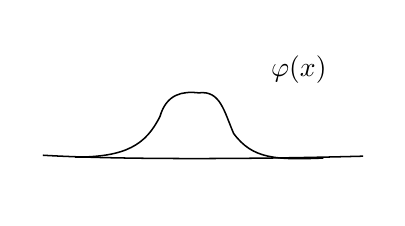
\begin{tikzpicture}[x=.12mm,y=-.12mm,line width=.55pt]\path[use as bounding box] (0,0) rectangle (370,180);
\draw (16,135) .. controls (100,140) and (246,139) .. (355,136);
\draw (50,137) .. controls (104,137) and (125,124) .. (140,94) .. controls (147,70) and (164,67) .. (181,69) .. controls (204,66) and (208,89) .. (218,112) .. controls (238,139) and (262,140) .. (313,138);
\node at (287,44) {$\varphi(x)$};
\end{tikzpicture}}
$S(x)$ can be $S(x)=px$.
\SourceFigure{GELFAND-P000041}{wave-packet}{Wavy and almost vertical strokes lie between rounded upper and lower contours, crossed by an almost horizontal stroke. Some individual connections at the ends and thickened parts cannot be distinguished securely.\par\smallskip\centering\color{black}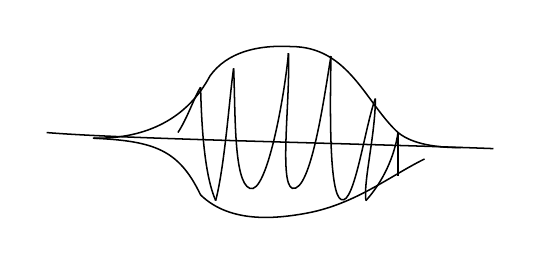
\begin{tikzpicture}[x=.12mm,y=-.12mm,line width=.55pt]\path[use as bounding box] (0,0) rectangle (505,220);
\draw (20,111) .. controls (105,118) and (335,122) .. (493,128);
\draw (69,117) .. controls (126,118) and (169,96) .. (193,51) .. controls (211,26) and (243,18) .. (279,20) .. controls (340,20) and (358,80) .. (392,111) .. controls (408,124) and (435,127) .. (459,127);
\draw (70,117) .. controls (134,120) and (160,129) .. (183,177) .. controls (215,208) and (265,202) .. (297,196) .. controls (348,186) and (385,156) .. (420,139);
\draw (159,111) .. controls (169,96) and (177,72) .. (183,63);
\draw (183,63) .. controls (184,104) and (187,156) .. (199,183);
\draw (199,183) .. controls (209,144) and (214,68) .. (218,43);
\draw (218,43) .. controls (220,92) and (218,163) .. (235,170) .. controls (253,178) and (272,72) .. (276,27);
\draw (276,27) .. controls (278,77) and (266,164) .. (280,170) .. controls (300,175) and (314,72) .. (321,30);
\draw (321,30) .. controls (320,90) and (319,177) .. (332,182) .. controls (346,188) and (357,104) .. (368,75);
\draw (368,75) .. controls (368,113) and (355,164) .. (358,183);
\draw (358,183) .. controls (376,163) and (388,137) .. (392,111);
\draw (392,111) -- (392,157);
\end{tikzpicture}}
\par\noindent\begin{minipage}{\linewidth}
Oscill. (rapid), \textcolor{orange!65!black}{[пропод.]}\ $\varphi$.
\Unclear{GELFAND-P000041}{caption-contraction}{After “Oscill. (rapid)” the manuscript writes пропод. Its expansion is uncertain. It is followed by $\varphi$.}
\end{minipage}\par

\Needspace{5\baselineskip}
\SourcePage{GELFAND-P000042}{unlabelled}
Seek the asympt. as $h\to0$ in the form
\begin{equation*}
\Psi=e^{\frac{i}{h}a(x,t)}.
\end{equation*}
$a$ --- a complex fn.
Substitute and obtain a seq. of asympt. formulas for the solution of the prob.
The first 2 terms have the form
\par\noindent\begin{minipage}{\linewidth}
\begin{equation*}
\Psi(x,t)=
\frac{\varphi(X(x,t)}{\sqrt{\frac{\partial x(X,t)}{\partial X}}}
e^{\frac{i}{h}\left(S(X(x,t))+\int p\,dx\right)+O(h)}
\end{equation*}
\EvidenceBlock{GELFAND-P000042}{amplitude-delimiter}{There is one closing parenthesis after $t$ in the numerator.}{Manuscript notation.}
\Unclear{GELFAND-P000042}{remainder}{The entry $+O(h)$ is on the raised line after the phase parenthesis; there is no separate lower line for it.}
\Unclear{GELFAND-P000042}{amplitude-jacobian}{The first rounded sign in the numerator beneath the radical resembles $D$ / $\partial$; the denominator shows $\partial X$. The upper argument is written $(X,t)$.}
\end{minipage}\par
[From the denominator: --- from unit.; see Titchmarsh and Landau.]
$\varphi$ --- given init. amplitude.
$X$ at $t=0$ $=x$.
\par\noindent\begin{minipage}{\linewidth}
$\underset{(x,t)}{X}$ --- [cancelled: a point from which one must].
\Unclear{GELFAND-P000042}{cancelled-origin}{Beneath the cancellation: точка, из к-рой надо / наше (a point from which one must / ours); the final letters are crossed by the stroke.}
\end{minipage}\par
Classical init. condition.
\par\noindent\begin{minipage}{\linewidth}
\begin{equation*}
p=\dot{x},\qquad \dot{x}=\frac{\partial S}{\partial x}
\end{equation*}
\Unclear{GELFAND-P000042}{classical-initial-signs}{A dot is visible over each $x$ / $X$. The lower sign after $\partial S$ resembles $X$ / $x$; its case is not secure. No separate subscript is visible on the first sign.}
\end{minipage}\par
\par\noindent\begin{minipage}{\linewidth}
$S$ is given at the init. instant.
$n$-dim. \textcolor{orange!65!black}{пв. / пб.}
\Unclear{GELFAND-P000042}{dimensional-abbreviation}{After $n$-dim. is a short joined abbreviation resembling пв. / пб.; it is not expanded.}
\end{minipage}\par
\SourceFigure{GELFAND-P000042}{phase-figure}{An almost horizontal line crosses a vertical one; an arch lies above them, with two vertical strokes from it. $X$ is below the left stroke; $x$ stands between the strokes. Inside: time $t$. An inclined stroke rises rightwards from the left junction, with a thickened start; its arrow direction is not established.\par\smallskip\centering\color{black}\begin{tikzpicture}[x=.12mm,y=-.12mm,line width=.55pt]\path[use as bounding box] (0,0) rectangle (550,320);
\draw (28,223) .. controls (149,231) and (347,200) .. (528,193);
\draw (172,58) .. controls (167,119) and (164,210) .. (170,287);
\draw (206,184) .. controls (245,139) and (278,112) .. (302,107) .. controls (364,92) and (431,107) .. (488,141);
\draw (288,111) -- (390,76);
\draw (287,111) -- (294,211);
\draw (487,145) -- (487,155);\draw (487,162) -- (488,174);\draw (488,180) -- (489,192);
\draw[line width=1pt] (281,105) -- (297,115);\draw[line width=1pt] (288,102) -- (287,123);
\node at (285,271) {$X$};\node at (390,242) {$x$};\node at (370,145) {time $t$};
\end{tikzpicture}}
The formula is quasiclassical, valid when the Jacob. $\neq0$.
\underline{Quasicl.} --- when this formula holds.
\begin{equation*}
\ddot{x}=-\frac{\partial U}{\partial x}
\end{equation*}
classical mechanics ($x$ --- vector).
In quantum mech., $\forall t$ there is a wave fn. $\Psi$.
$|\Psi|^2$ --- prob.
\par\noindent\begin{minipage}{\linewidth}
Eqn. of motion --- Schröd.
\begin{equation*}
\frac{i}{h}\frac{\partial\Psi}{\partial t}
=\Delta\Psi-\frac{U(x)}{h^2}\Psi
\end{equation*}
\Unclear{GELFAND-P000042}{schrodinger-factor}{The repeated equation has $i/h$ at left and $U(x)/h^2$ at right; the two fractions are separately visible.}
\end{minipage}\par
(if there is no $i$, then it is the heat eqn.;
if initially at a point, it later spreads out).
Connected with the asympt. of eigenvalues.
$\left.\Psi\right|_{t=0}$ is given. $\Psi(x)$
\SourceFigure{GELFAND-P000042}{terminal-line}{A long almost horizontal stroke with a thickened right end follows $\Psi(x)$. There is no caption over it or secure arrowhead.\par\smallskip\centering\color{black}\begin{tikzpicture}[x=.12mm,y=-.12mm,line width=.55pt]\path[use as bounding box] (0,0) rectangle (335,115);
\draw (0,71) .. controls (103,69) and (175,82) .. (280,75);
\draw[line width=.9pt] (276,73) -- (284,76);
\end{tikzpicture}}

\Needspace{5\baselineskip}
\SourcePage{GELFAND-P000043}{22}
$S(x)=px$, then the de Broglie formula.
\begin{equation*}
\frac{\partial S}{\partial x}=p
\end{equation*}
\par\noindent\begin{minipage}{\linewidth}
Usual method of finding the asympt. --- seek the soln. in the form
\begin{equation*}
e^{\frac{i}{h}S_0(x^t)+S_1(x^t)+hS_2(x^t)+\cdots}
\end{equation*}
\Unclear{GELFAND-P000043}{exponent-variables}{A raised sign with a crossbar resembling $t$ stands over $x$ in all three arguments; readings $x^t$ / $\dot{x}$. The subscript of the second $S$ is blotted: $S_1$ / $S_0$.}
\end{minipage}\par
With respect to time [inserted above: diff.] $\frac{1}{h^2}$ \ldots
The leading term must be sought as $e^{\frac{i}{h}S_0(x)}$.
If $S$ is real, then oscill.; if complex, then there is decay.
Obtain a 1st-order eqn., and the 1st fn. is real, and obtain oscill.
Must take the amplit., hence 2 terms.
Now must choose init. data for this asympt.
\par\noindent\begin{minipage}{\linewidth}
$\Omega$ / $\delta$ is not allowed, since there are many extraneous frequencies (strongly localized).
\Unclear{GELFAND-P000043}{localized-datum}{$\Omega$ or $\delta$: a loop with a horizontal lower stroke and a long left tail.}
\end{minipage}\par
\begin{equation*}
\varphi(x,t)e^{\frac{i}{h}S(x,t)}
\end{equation*}
if substituted there, then for $S$ a 1st-order eqn.
\begin{equation*}
\frac{\partial S}{\partial t}
=H\left(x,\frac{\partial S}{\partial x}\right),
\qquad H=U(x)+\frac{\dot{x}^2}{2}
\end{equation*}
to which an ordinary eqn. corresponds.
$\varphi$ --- density of the dyn. syst. (how they move according to class. mech.).
Must take $x$ and find $X$ for it, so that
our eqn. comes from $X$ to $x$ after $t$.
The points carry $\varphi$ with them.
\SourceFigure{GELFAND-P000043}{trajectory}{A bending curve has $X$ below the left junction and $x$ at its right end. A thick inclined stroke passes through the left junction. Its arrowhead or direction is not established.\par\smallskip\centering\color{black}\begin{tikzpicture}[x=.10mm,y=-.10mm,line width=.55pt]\path[use as bounding box] (0,0) rectangle (465,320);
\draw (30,275) .. controls (55,206) and (94,149) .. (130,110) .. controls (199,82) and (352,77) .. (433,129);
\draw[line width=.85pt] (130,110) -- (232,27);
\draw[line width=.85pt] (21,269) -- (37,280);
\draw[line width=.85pt] (429,124) -- (437,132);
\node at (180,145) {$X$};\node at (429,160) {$x$};
\end{tikzpicture}}
$\dot{x}$ is given from $x$ (the dyn. syst. is given).
For small $t$, single-valued.
\begin{equation*}
\Psi=e^{iH}
\end{equation*}
unit.
$\mathcal{D}$ --- the Jacob. is added for unitarity.
$e$ --- the phase factor rotates with varying amplitude.
Maslov's work, when $t$ is arbitrary rather than small.
\par\noindent\begin{minipage}{\linewidth}
$t=0$, Jacob. [an entry is cancelled] $=1$ (identity transf.).
\Unclear{GELFAND-P000043}{cancelled-jacobian}{A heavily cancelled expression after Jacob. and before $=1$; the individual signs are not established.}
\end{minipage}\par
The wave fn. of the oscillator. Pendulum.
\SourceFigure{GELFAND-P000043}{oscillator}{A parabolic arch, oscillating contour, almost horizontal stroke and central stroke intersect. Visible labels: $\varphi$, $0$, $x$; a small upper sign resembles $\xi$, but its lower part joins the curve. Captions: in class. mech. wave fn.; $\exp$ decay. Exact connections of dense strokes and the number of oscillations are not established.\par\smallskip\centering\color{black}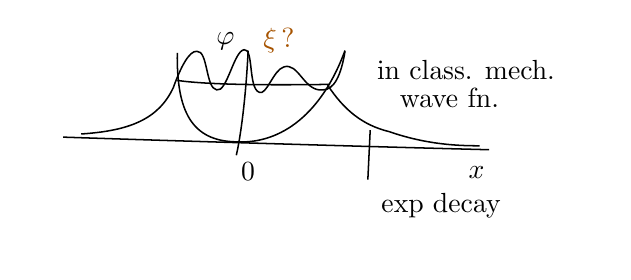
\begin{tikzpicture}[x=.10mm,y=-.10mm,line width=.55pt]\path[use as bounding box] (0,0) rectangle (730,285);
\draw (45,139) .. controls (193,144) and (430,151) .. (586,155);
\draw (190,32) .. controls (189,106) and (208,144) .. (265,145) .. controls (323,148) and (374,108) .. (403,29);
\draw (68,135) .. controls (128,131) and (166,117) .. (185,76) .. controls (194,51) and (205,29) .. (215,30);
\draw (215,30) .. controls (229,29) and (226,77) .. (240,79) .. controls (253,83) and (262,29) .. (275,28) .. controls (287,26) and (280,77) .. (294,82) .. controls (303,87) and (312,54) .. (325,50) .. controls (344,43) and (351,82) .. (375,79) .. controls (389,79) and (398,61) .. (403,30);
\draw (190,67) .. controls (232,73) and (315,73) .. (384,72);
\draw (381,73) .. controls (402,105) and (426,124) .. (459,132) .. controls (508,149) and (549,150) .. (574,150);
\draw (280,29) .. controls (278,71) and (273,126) .. (265,162);
\draw (435,130) -- (432,193);
\node at (251,17) {$\varphi$};\node[text=orange!65!black] at (319,17) {$\xi\,?$};
\node at (280,183) {$0$};\node at (570,184) {$x$};
\node[anchor=west] at (431,54) {in class. mech.};\node[anchor=west] at (460,89) {wave fn.};
\node at (525,226) {$\exp$ decay};
\end{tikzpicture}}

\Needspace{5\baselineskip}
\SourcePage{GELFAND-P000044}{unlabelled}
If $t$ is large, it may happen that
the curve of init. data ($n$-dim. пв.) moves.
\SourceFigure{GELFAND-P000044}{folded-data}{Upper-left drawing: several bending arches cross inclined strokes, an almost horizontal line and a dense almost vertical bundle. Small tips appear at the upper-left end and inside the bundle; some individual connections overlap.\par\smallskip\centering\color{black}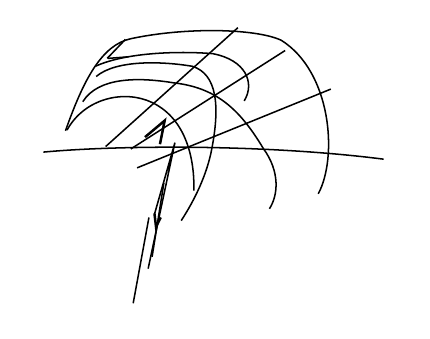
\begin{tikzpicture}[x=.10mm,y=-.10mm,line width=.55pt]\path[use as bounding box] (0,0) rectangle (475,360);
\draw (20,158) .. controls (117,149) and (304,148) .. (452,167);
\draw (48,131) .. controls (71,66) and (94,22) .. (131,14) .. controls (201,-1) and (290,1) .. (322,16) .. controls (386,56) and (394,165) .. (369,211);
\draw (70,94) .. controls (90,62) and (142,63) .. (185,70) .. controls (239,76) and (269,103) .. (299,153) .. controls (321,183) and (318,213) .. (307,230);
\draw (50,130) .. controls (72,90) and (122,78) .. (158,95) .. controls (206,118) and (212,177) .. (211,207);
\draw (87,62) .. controls (113,40) and (173,43) .. (209,49) .. controls (241,59) and (244,100) .. (234,153) .. controls (228,186) and (212,219) .. (195,245);
\draw (86,49) .. controls (128,30) and (199,30) .. (235,33) .. controls (277,41) and (289,70) .. (275,93);
\draw (101,39) -- (124,15);\draw (102,39) -- (128,37);
\draw (99,151) -- (267,0);
\draw (131,154) -- (327,29);
\draw (139,178) -- (385,78);
\draw (161,237) -- (187,146) -- (153,306);
\draw (173,197) -- (158,291);\draw (154,241) -- (134,350);
\draw[line width=.9pt] (149,139) -- (174,118) -- (168,148);
\draw[line width=.9pt] (169,241) -- (163,253) -- (161,236);
\end{tikzpicture}}
\par\noindent\begin{minipage}{\linewidth}
If there is a vertical tangent, then $\mathcal{D}=0$,
but afterwards there are 2 points and the formula is retained [(!) / (?)], but
must add terms over the points $\gamma_j$ / $n_j$ --- an integer.
\Unclear{GELFAND-P000044}{preserved-punctuation}{After retained, a small parenthesized sign with a separate lower dot: (!) / (?). Its upper part is blotted.}
\Unclear{GELFAND-P000044}{phase-integer}{$\gamma_j$ or $n_j$: the upper sign has a loop and two raised strokes; $j$ lies below. The following entries resemble $n_j$.}
\end{minipage}\par
\par\noindent\begin{minipage}{\linewidth}
\begin{equation*}
\int p\,dx)+i\,\frac{\pi}{2}n_j
\end{equation*}
[A sign between $i$ and $\pi/2$ is cancelled.]
\Unclear{GELFAND-P000044}{cancelled-phase-sign}{A sign between $i$ and $\pi/2$ is heavily cancelled; the readings $+$ / $-$ are not securely established.}
\end{minipage}\par
\uwave{Maslov's result} --- the \uuline{$n_j$} have been found.
$n_j=\pm1$ from general considerations.
Go around the branch point in the complex plane;
this can determine $\oplus$ or $\ominus$.
All results also apply in \underline{optics}.
\SourceFigure{GELFAND-P000044}{optical-rays}{Several inclined rays cross a bending envelope. A thick arrow points downwards to the right at the upper tangency. Short crossing strokes lie on the lower-right branch; their connection to the envelope is uncertain.\par\smallskip\centering\color{black}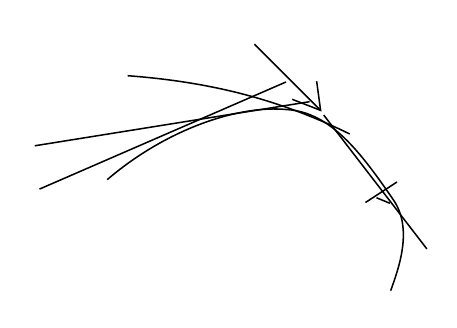
\begin{tikzpicture}[x=.10mm,y=-.10mm,line width=.55pt]\path[use as bounding box] (0,0) rectangle (510,345);
\draw (9,150) -- (358,94);
\draw (15,205) -- (328,69);
\draw (127,61) .. controls (233,69) and (319,91) .. (409,135);
\draw (101,193) .. controls (177,128) and (269,98) .. (329,104) .. controls (385,107) and (424,160) .. (464,218) .. controls (490,255) and (471,306) .. (461,334);
\draw (288,21) -- (372,105);\draw (336,91) -- (372,105) -- (367,68);
\draw (376,111) -- (507,281);
\draw (429,222) -- (469,196);\draw (443,216) -- (460,223);
\end{tikzpicture}}
The rays envelop a curve.
We shall follow the phase along a ray.
For small $\lambda$ --- a phase jump of $\pi/2$ at the point of tangency.
\underline{Answer} $n_j$ --- the Morse index.
\SourceFigure{GELFAND-P000044}{trajectory-figure}{The $p$ axis points upwards and the horizontal axis rightwards. A family of bending and almost vertical strokes; $x_1$, $x_2$, $X$. Captions: curve of init. data; classical; degenerate here; after time $t$; after $t$; conj. points. A small dense sign is above the central vertical stroke; its reading and some individual intersections are not established.\par\smallskip\centering\color{black}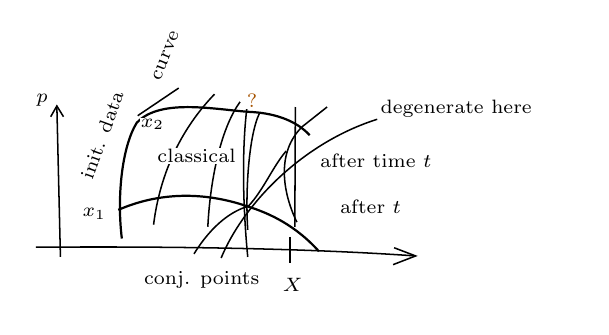
\begin{tikzpicture}[x=.065mm,y=-.065mm,line width=.55pt,every node/.style={font=\scriptsize,fill=white,inner sep=.4pt}]\path[use as bounding box] (0,0) rectangle (1080,545);
\draw (16,429) .. controls (277,427) and (545,431) .. (758,446);
\draw (716,430) -- (758,446) -- (714,463);
\draw (64,448) -- (57,153);\draw (45,174) -- (57,153) -- (70,174);
\node at (28,142) {$p$};
\draw[line width=.8pt] (184,412) .. controls (174,331) and (184,233) .. (213,186) .. controls (260,135) and (375,162) .. (441,165) .. controls (483,168) and (524,181) .. (551,210);
\draw[line width=.8pt] (177,356) .. controls (269,316) and (359,325) .. (429,349) .. controls (474,363) and (524,387) .. (569,437);
\draw (215,172) -- (295,118);
\draw (246,385) .. controls (256,304) and (288,210) .. (365,130);
\draw (352,389) .. controls (356,306) and (375,200) .. (415,145);
\draw (430,144) .. controls (418,229) and (420,345) .. (430,448);
\draw (453,167) .. controls (432,210) and (425,320) .. (430,395);
\draw (523,155) -- (522,389);
\draw (526,380) .. controls (497,320) and (486,242) .. (537,193) -- (585,155);
\draw (431,349) .. controls (461,317) and (478,273) .. (505,241);
\draw (378,450) .. controls (422,344) and (537,225) .. (683,179);
\draw (325,442) .. controls (362,382) and (402,357) .. (431,349);
\draw (513,409) -- (513,460);
\node at (130,363) {$x_1$};\node at (244,189) {$x_2$};\node at (518,503) {$X$};
\node[text=orange!65!black] at (435,143) {$?\!$};
\node[rotate=70] at (145,210) {init. data};
\node[rotate=68] at (270,55) {curve};
\node[anchor=west] at (250,251) {classical};
\node[anchor=west] at (686,158) {degenerate here};
\node[anchor=west] at (568,260) {after time $t$};\node[anchor=west] at (607,350) {after $t$};
\node at (340,493) {conj. points};
\end{tikzpicture}}
A trajectory is a soln. of a variational problem by
the principle of least action.
\begin{gather*}
\delta u=0\\
\delta^2u
\end{gather*}
\par\noindent\begin{minipage}{\linewidth}
a quadratic form. It has an index [a word is cancelled]
(number of neg. squares).
\Unclear{GELFAND-P000044}{cancelled-index}{A short word left of (number of neg. squares) is cancelled by dense strokes; its reading is not established.}
\end{minipage}\par
\par\noindent\begin{minipage}{\linewidth}
Or [a word is cancelled] the number of conjugate points.
\Unclear{GELFAND-P000044}{cancelled-conjugate}{A word above number of conjugate points is covered by several horizontal strokes; its reading is not established.}
\end{minipage}\par
The 1st part of \underline{Leray}'s work is devoted to related questions.
\par\noindent\begin{minipage}{\linewidth}
Next time Povzner Yang Lee and \textcolor{orange!65!black}{Brushlin [Брушлин]}.
\Unclear{GELFAND-P000044}{next-speakers}{The line reads “Yang Lee”. Above “Lee” is a short Russian addition resembling группам [to groups]. The final surname is provisionally read as Брушлин [Brushlin].}
\end{minipage}\par

\Needspace{5\baselineskip}
\SourcePage{GELFAND-P000045}{23}
\underline{Berezin.}
\begin{equation*}
H=\frac{p^2}{2}+V(x)
\end{equation*}
(e.g. $V$ grows).
Let the surfaces $p^2+V(x)=\mathrm{const}$ all be bounded.
\par\noindent\begin{minipage}{\linewidth}
Then the asympt. of eigenvalues [an abbreviation is cancelled]:
\Unclear{GELFAND-P000045}{cancelled-eigenfunction}{The cancelled abbreviation before values resembles ф-й / ф-и (fns.); horizontal strokes cross the upper letters.}
\end{minipage}\par
\par\noindent\begin{minipage}{\linewidth}
the volume of the region where $H\leq n\pi h$ --- the asymptotic
[a word is cancelled] of the eigenvalues.
\Unclear{GELFAND-P000045}{cancelled-asymptotic}{A short word between asymptotic and eigenvalues is covered by dense ink; its reading is not established.}
\end{minipage}\par
\par\medskip{\centering\rule{12mm}{.45pt}\enspace$\cdot$\enspace\rule{15mm}{.45pt}\par}\medskip
\underline{Gelfand I.}
\begin{equation*}
-y''+p(x)y=\lambda y
\end{equation*}
\SourceFigure{GELFAND-P000045}{wavefunction-diagram}{A horizontal segment with short end strokes and labels $0$, $\pi$. One arch lies above the segment; another curve begins above it, crosses it, and falls below. A dense junction lies near the right end; the nearby underline under zero at the endpoints is crossed out.\par\smallskip\centering\color{black}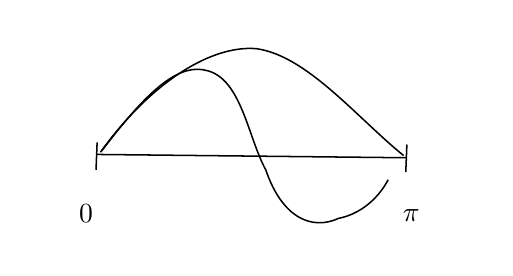
\begin{tikzpicture}[x=.14mm,y=-.14mm,line width=.55pt]
\path[use as bounding box] (0,0) rectangle (415,200);
\draw (63,115) -- (344,118);
\draw (63,104) -- (62,129);\draw (344,106) -- (343,131);
\draw (66,113) .. controls (113,48) and (167,16) .. (207,19) .. controls (253,25) and (298,81) .. (341,116);
\draw (67,112) .. controls (111,54) and (138,32) .. (163,39) .. controls (194,47) and (200,100) .. (216,129) .. controls (231,173) and (258,184) .. (282,173) .. controls (302,169) and (318,155) .. (327,138);
\node at (53,169) {$0$};\node at (348,170) {$\pi$};
\end{tikzpicture}}
\underline{Zero at the endpoints} [the underline is crossed out].
\par\noindent\begin{minipage}{\linewidth}
$p=0$, eigenfns., $\lambda=-n^2$.
\Unclear{GELFAND-P000045}{lambda-sign}{In $\lambda=-n^2$, a separate horizontal stroke is visible between the equality sign and $n$; the minus is retained.}
\end{minipage}\par
Claim. The 1st eigenfn. has no zeros (Morse index 1).
The 2nd --- ditto --- has one zero.
This holds for $\forall$ eqn.
The zeros interlace.
A more precise theorem. If $y_0,\ldots,y_n$ are eigenfns.,
then
\begin{equation*}
\sum_{i=1}^{n}a_i y_i(x)
\end{equation*}
will have $\leq n$ zeros!!
(resembles polynomials).
\par\noindent\begin{minipage}{\linewidth}
[A cancelled determinant:]
\begin{equation*}
\det\begin{vmatrix}
y_0(x)&y_1&\cdots\\
y_0'(x)&y_1'&\\
\vdots&\vdots&\\
y_0^{(n)}(x)&y'(x)&
\end{vmatrix}
\end{equation*}
\Unclear{GELFAND-P000045}{cancelled-determinant}{The lower second entry of the cancelled determinant resembles $y\prime(x)$ / $y_1^{(n)}(x)$; its subscript and derivative order are not established.}
\end{minipage}\par
\par\noindent\begin{minipage}{\linewidth}
This is equiv. to the condition
\begin{equation*}
\begin{vmatrix}
y_0(x_0)&y_1(x_1)&\cdots\\
y_0'(x_0)&y_1'(x_1)&\cdots\\
\vdots&\vdots&\\
y_0^{(n)}(x_0)&y_1'(x_1)&
\end{vmatrix}\neq0
\end{equation*}
\Unclear{GELFAND-P000045}{mixed-determinant}{The upper sign of $y_1\prime(x_1)$ in the second entry of the second row is overwritten. A single raised stroke is visible in the lower second entry: $y_1\prime(x_1)$; a possible order $(n)$ is not established.}
\end{minipage}\par
\par\noindent\begin{minipage}{\linewidth}
Or
[Above the following determinant:] this is the 1st eigenfn. of the 2nd-order eqn., which is $\neq0$.
\begin{equation*}
\begin{vmatrix}
y_0(x_0)&y_1(x_0)&\cdots\\
y_0(x_1)&y_1(x_1)&\cdots\\
\vdots&\vdots&\\
y_0(x_n)&y_0(x_n)&
\end{vmatrix}\neq0
\end{equation*}
\Unclear{GELFAND-P000045}{value-determinant}{In the second entry of the bottom row the subscript is rounded, like $y_0$ in the first column. The dot above it aligns with the vertical ellipsis; a separate derivative stroke is uncertain.}
\end{minipage}\par
Hence a linear comb. has $\leq n$ zeros if $x_0<x_1<\cdots<x_n$.
\par\noindent\begin{minipage}{\linewidth}
Petrov. So that
\begin{equation*}
\begin{aligned}
\frac{\partial^2u}{\partial x_1^2}
-\frac{\partial^2u}{\partial x_2}-\cdots
+\left(p(x_1)+p(x_2)\ldots+p(x_n)\right)u&={}\\
&=\lambda u
\end{aligned}
\end{equation*}
\Unclear{GELFAND-P000045}{petrov-equation}{The first denominator is $x_1^2$; the second shows $x_2$ without a square. At the right edge: $u=$; below, another equality sign before $\lambda u$. Both signs are retained.}
\end{minipage}\par
Eigenfns., the variables separate.
Eigenfns. $u_1(x_1)u_2(x_2)\ldots u_n(x_n)$.
The 1st eigenfn. $\neq0$.

\Needspace{5\baselineskip}
\par\noindent\begin{minipage}{\linewidth}
\SourcePage{GELFAND-P000046}{unlabelled}
\par\medskip{\centering\rule{12mm}{.45pt}\enspace$\cdot$\enspace\rule{15mm}{.45pt}\par}\medskip
\uwave{Planned}. [Number and initials unclear] Bernstein and S. Gilfand.
\Unclear{GELFAND-P000046}{planned-speakers}{The first row begins with a long looped sign, then И / Н before Бернштейн. Readings: $1^\circ$ I. Bernstein and S. Gilfand / F. N. Bernstein and S. Gilfand / $1^\circ$ I. Bernstein and S. Gelfand. Full names are not established.}
\end{minipage}\par
[Separately at the right:] \uwave{Dyson}.
$2^\circ$. Novikov, on the work of \uwave{Adams}.
$3^\circ$. Dynkin.
$4^\circ$. Vinberg.
$5^\circ$. Pyatetskii-Shapiro.
\par\noindent\begin{minipage}{\linewidth}
[Cancelled.]
\Unclear{GELFAND-P000046}{cancelled-heading}{The short cancelled and doubly underlined heading before Pyat.-Shapiro resembles Пят. (Pyat.); dense strokes cover the earlier writing.}
\end{minipage}\par
\underline{Pyat.-Shapiro}.
Problem of Klein and Serre.
Consider the gr. of integer matrices of order $n$, $\Gamma(n)$, with $\det=1$.
[Cancelled: How]
describe all subgrs. $\Gamma'$ of finite index?
\underline{Ex.}
\par\noindent\begin{minipage}{\linewidth}
\begin{equation*}
\Gamma(n,N),\qquad A\equiv E\pmod N
\end{equation*}
\Unclear{GELFAND-P000046}{congruence-index}{A small inscription below $\Gamma(n,N)$ resembles $\lambda ij$ / $i,j$; below $A\equiv E$: probably не гр. (not gr.), possibly на гр. (on gr.). The letters and the attachment of the small inscription to the formula are not established.}
\end{minipage}\par
(on the diag., congruent to $1$; off the diag., divisible by $N$).

\Needspace{5\baselineskip}
\SourcePage{GELFAND-P000047}{35}
Are these all the subgroups?
Does $\Gamma'$ always contain $\Gamma(n,N)$
(a congruence subgr.).
For $n=2$ this is false (Klein).
$n\geq3$, this is true (Serre).
\underline{Connection with Lie groups.}
Consider the matrices
\SourceFigure{GELFAND-P000047}{elementary-stencil}{Matrix schematic.\par\smallskip
\centering\color{black}
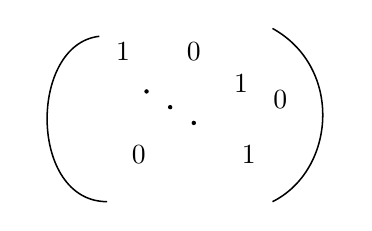
\begin{tikzpicture}[x=1mm,y=-1mm,line width=.55pt]
\draw (9,2) .. controls (0,3) and (0,23) .. (10,23);
\draw (31,1) .. controls (40,6) and (39,19) .. (31,23);
\node at (12,4) {$1$};\node at (21,4) {$0$};
\node at (27,8) {$1$};\node at (32,10) {$0$};
\fill (15,9) circle (.28);\fill (18,11) circle (.28);\fill (21,13) circle (.28);
\node at (14,17) {$0$};\node at (28,17) {$1$};
\end{tikzpicture}}
\par\noindent\begin{minipage}{\linewidth}
[Cancelled symbol.]
\Unclear{GELFAND-P000047}{cancelled-elementary}{A cancelled and overwritten sign before the elementary-matrix notation resembles $E$; the underlying strokes are not established.}
\end{minipage}\par
\par\noindent\begin{minipage}{\linewidth}
$E_{ke}=(\mathrm{id.}+E_{ke})$.
\Unclear{GELFAND-P000047}{elementary-matrix}{The same $E$-shaped sign occurs on both sides of the equality; its second subscript resembles $e$ / $\ell$. Readings $E_{ke}=(\text{id.}+E_{ke})$ / $e_{k\ell}=(\text{id.}+E_{k\ell})$. The schematic matrix retains the visible ones, zeros and dots; unwritten entries have not been supplied.}
\end{minipage}\par
\underline{The gr. $\Gamma(n)$ is generated by them}.
Take these matrices and their conjugates and raise them to the power $N$:
$E_{ke}^{N}$, $\Gamma^{N}$.
For $n=2$ it has infinite index;
$n\geq3$, finite index.
$\Gamma/\Gamma^{N}$.
\fbox{$n=2$}
\par\noindent\begin{minipage}{\linewidth}
$N=2,3,4,5$ is finite, 6 \textcolor{orange!65!black}{commut. / коннут. [коммут. / коннут.; uncertain abbreviation]}
\Unclear{GELFAND-P000047}{surface-abbreviation}{After 6, the abbreviation коммут. / коннут. (commut. / коннут.; uncertain reading). Its initial letter has separate vertical and angled strokes. Below: $p=p(N)$; the letter resembles $p$. The abbreviation is not expanded.}
\end{minipage}\par
$\Gamma/\Gamma^{N}=$ fund. gr. of a surface,
$p=p(N)$, a simple formula.
Serre, Lazard, Bass (1964).
\par\noindent\begin{minipage}{\linewidth}
Consider $a\equiv b\ (N)$, then for $n\geq3$ / $N\geq3$
there is a transf. $a\to b$ in $\Gamma/\Gamma^{N}$ (elem. transf.).
\Unclear{GELFAND-P000047}{rank-overwrite}{After then for, the sign before $\geq3$ is heavily overwritten: $n\geq3$ / $N\geq3$. Vertical strokes resembling capital $N$ are visible.}
\end{minipage}\par
Then cohomol. technique.

\underline{Gelfand.}
Tomorrow at the conf. on elem. particles, there will be a talk about
\par\noindent\begin{minipage}{\linewidth}
[Cancelled.]
\Unclear{GELFAND-P000047}{cancelled-particles}{A group designation before boxed $SU(3)$ is densely cancelled. Readings $SU(3)$ / $SU(2)$; the digit beneath the ink is not established.}
\end{minipage}\par
\fbox{$SU(3)$}.
Known particles are combined into groups, transforming into one another (multiplets).
Another repr. of $SU(3)$.
The idea $SU(2)\underset{\text{almost}}{\approx}SO(3)$.
[Above the line: fns., lin. comb.]
Combine by means of 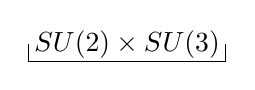
\begin{tikzpicture}[baseline=(product.base)]\node[inner xsep=2pt,inner ysep=1pt] (product) {$SU(2)\times SU(3)$};\draw (product.west) -- (product.south west) -- (product.south east) -- (product.east);\end{tikzpicture}.
The hypothesis is known also for $SU(6)$.
\underline{Remark} --- actually the Lorentz group (with par. translations)
(the Poincar\'e group).
[Cancelled: $SU(2)$] $\longrightarrow$ Poincar\'e gr.
Work of \underline{Todorov}.
\uwave{Kadyshevsky}, \uwave{Muradyan}, \uwave{Tavkhelidze}.
Instead of $SU(6)$ --- a 108-param. group.

\Needspace{5\baselineskip}
\SourcePage{GELFAND-P000048}{unlabelled}
Salam proposed a 144-param. group.
Fulton, Wess.
A 2-step gr. with a comm. normal divisor.
\par\noindent\begin{minipage}{\linewidth}
$SU(3)\otimes SU(2)$ in some sense.
\Unclear{GELFAND-P000048}{in-some-sense}{The abbreviation before смысле (sense) resembles как. or нек.}
\end{minipage}\par
Lorentz transf. --- complex matrices.
\begin{equation*}
\begin{pmatrix}\alpha&\beta\\\gamma&\delta\end{pmatrix},
\qquad \det=1
\end{equation*}
(spinor repr. of the Lorentz gr.).
\uwave{Poincar\'e} gr.\enspace\rule[-.28em]{.6pt}{1.4em}
\begin{equation*}
A=\begin{pmatrix}\alpha&\beta\\\gamma&\delta\end{pmatrix}
\end{equation*}
\uwave{Vector} --- Hermitian forms of order 2.
\begin{equation*}
H=\begin{pmatrix}a&b\\\bar b&c\end{pmatrix}
\end{equation*}
A vector in 4-dim. space; $a,c$ real, $b$ complex.
\begin{equation*}
H\to AHA^*
\end{equation*}
Lorentz, $\det$ is preserved.
Poincar\'e gr.
\begin{equation*}
\begin{pmatrix}A&H\\0&A^{*-1}\end{pmatrix}
\end{equation*}
\par\noindent\begin{minipage}{\linewidth}
This is a group for $H\geq0$ / $H=0$ rot. ($H$ adds).
$H=1$ --- par. transl.
\Unclear{GELFAND-P000048}{h-zero}{The condition on $H$ has an upper angled stroke and a lower horizontal stroke before $0$; readings $H\geq0$ / $H=0$.}
\end{minipage}\par
\par\noindent\begin{minipage}{\linewidth}
[Cancelled.]
\Unclear{GELFAND-P000048}{cancelled-group}{Before Matrix of order 4, a cancelled phrase begins gr.; the next word resembles Вращ. / Лоренца (rot. / Lorentz).}
\end{minipage}\par
Matrix of order 4.
\begin{equation*}
\underline{\begin{pmatrix}A&H\\0&A^{*-1}\end{pmatrix}}\otimes SU(3)
\end{equation*}
\par\noindent\begin{minipage}{\linewidth}
Obtain a semisimple gr. with \textcolor{orange!65!black}{solv.} (108-param.).
\Unclear{GELFAND-P000048}{group-abbreviation}{The abbreviation after with resembles разреш. (solv.); the ending is joined.}
\end{minipage}\par
One can describe what is \underline{needed} \underline{to} solve the theor. of elem. particles).

15/II\par\underline{Kazhdan}.
Palam.'s result in purely alg. terms.
\par\noindent\begin{minipage}{\linewidth}
Let $A$ be an integral domain [domain inserted above a cancelled word]
(ring without zero divisors), $I$ a prim. ideal.
\Unclear{GELFAND-P000048}{domain-cancellation}{Область [domain] is inserted above a cancelled word; the candidate is кольцо [ring]. The dense strokes do not establish the whole word. The following целостности [integral, in integral domain] (ring without zero divisors) is legible.}
\end{minipage}\par
\par\noindent\begin{minipage}{\linewidth}
\begin{equation*}
I\supset J
\end{equation*}
[Beneath $J$:] prime.
And let $J\supset I^2$ [cancelled: $\neq$] $0$.
\Unclear{GELFAND-P000048}{ideal-powers}{$I$ is introduced as a prim. ideal; prime is written beneath $J$ in $I\supset J$. Next: $J\supset I^2$, with a cancelled sign resembling $\neq$ before $0$. The letters and cancellation are retained.}
\end{minipage}\par
Every such ideal is given by diff. \underline{opers. of \underline{order 1.}}

\Needspace{5\baselineskip}
\par\noindent\begin{minipage}{\linewidth}
\SourcePage{GELFAND-P000049}{36}
A diff. oper. is a $A$ / $K$ / $k$-lin. oper.
\Unclear{GELFAND-P000049}{linear-glyph}{The heavily overwritten sign before -lin. resembles $A$ with a projecting upper stroke. $K$ and $k$ remain possible.}
\end{minipage}\par
\par\noindent\begin{minipage}{\linewidth}
\begin{equation*}
D(a\cdot b)=aD(b)+D(a)b
\end{equation*}
\Unclear{GELFAND-P000049}{product-comma}{Below the multiplication dot in the argument of $D$ is a separate comma-like mark.}
\end{minipage}\par
An ideal is the zero of some collection of diff. opers.
Let $A/J^2$ (of order 1 because of $J^2$).
An operator with values in the ring $A/J$ instead of in the original ring.
Diff. everywhere, and the ans. on a subset.
$aD(b)$ --- multiplication by $a$.
On $J$ the oper. is $A$-linear [below: diff.].
Conversely, every $A$-lin. oper. on $J$
\par\noindent\begin{minipage}{\linewidth}
[Cancelled sign before $J$]:
\Unclear{GELFAND-P000049}{cancelled-map-strokes}{To the left of $J$, three dense, nearly vertical strokes with a loop are cancelled, followed by a colon. An individual underlying letter is not established.}
\begin{equation*}
J\overset{f}{\longrightarrow}A/J
\end{equation*}
\end{minipage}\par
Then it can be multiplied by an elem. $b$, again lin.
[Above: $bf$.]
$\exists b$ such that $bf$ extends to a diff. of the whole ring.
Everything follows from this.
\par\noindent\begin{minipage}{\linewidth}
We shall consider $J(2)$ / $J(\xi)$ / $J(\ell)$ over the field of fractions.
\Unclear{GELFAND-P000049}{field-notation}{The parenthesized sign after $J$ resembles $2$ / $\xi$ / $\ell$, followed by over the field of fractions. Readings $J(2)$ / $J(\xi)$ / $J(\ell)$.}
\end{minipage}\par
Functionals exist, appar. $J$ lies in the ring of fractions.
\par\noindent\begin{minipage}{\linewidth}
Multiply by $b$ (since there are no zero divisors, then [a short sign is cancelled] ring of fr.).
\Unclear{GELFAND-P000049}{cancelled-field-symbol}{A short densely cancelled sign between then and ring of fr.; its reading is not established.}
\end{minipage}\par
If $A/J$ is a field, then $\forall$ functional extends to a diff.
(Need to take the localization of $A/J$).
There is a map of the field
\begin{equation*}
A/J\longrightarrow A
\end{equation*}
[Beneath the arrow: hom.]
such that the reverse hom. is the identity.
\begin{equation*}
A/J\longrightarrow A\longrightarrow A/J
\end{equation*}
\par\noindent\begin{minipage}{\linewidth}
[Cancelled.]
\Unclear{GELFAND-P000049}{cancelled-word}{The cancelled heading before For now, arb. resembles Док-во. (Proof.); its reading remains uncertain beneath the strike.}
\end{minipage}\par
For now, arb.
$A/J\subset A$, $J\subset A$.
Any elem. decomposes into a $\Sigma$ ($\Sigma$ as a lin. space).

\Needspace{5\baselineskip}
\SourcePage{GELFAND-P000050}{unlabelled}
On $J$ it is already given.
A lin. map $J\to A/J$ extends.
\par
On the whole [of it], $0$.
\par
A transcend. elem. anywhere.
\par\noindent\begin{minipage}{\linewidth}
\begin{gather*}
y\to\hat y,\qquad x^2=y\\
\hat x'^{\,2}-\hat y=i_1;\qquad
\hat x=\hat x'+i_2;\\
\hat x^2=\hat x'^{\,2}+2\hat x'i_2
=\hat y+2\hat xi_2+i_1
\end{gather*}
\Unclear{GELFAND-P000050}{square-expansion}{The expansion has no $i_2^2$. The multiplier is $\hat x\prime$ in the first equality and $\hat x$ without a prime in the second. Both readings are retained.}
\end{minipage}\par
Hence $i_2$ is found (since $A/J$ is a field).
Instead of $I$, $J$ was written, and conversely.
\par\medskip{\centering\rule{12mm}{.45pt}\enspace$\cdot$\enspace\rule{15mm}{.45pt}\par}\medskip
General form of a diff. oper. in the polynomial ring.
\begin{equation*}
\sum P_i(x_1,\ldots,x_n)\frac{\partial}{\partial x_i}
\end{equation*}
$P_i$ are polynomials.
\uwave{Alg. theory of diff. eqns.} \uwave{over an arb. field}.
Dieudonn\'e, Grothendieck: in alg. problems, passed to an arb. field.
\par\noindent\begin{minipage}{\linewidth}
\underline{Ordinary eqn.}
\begin{gather*}
\frac{dx}{dt}=P(x,y)\\
\frac{dy}{dt}=Q(x,y)
\end{gather*}
\Unclear{GELFAND-P000050}{overwritten-numerator}{The letter in the numerator of the first equation is heavily overwritten; the visible candidate is $dx$, and the earlier letter is not established.}
\end{minipage}\par
$t$ is replaced by a local ring at $\forall$ point ($t$ a local parameter).
\begin{gather*}
x=\sum a_k t^k\\
y=\sum b_k t^k
\end{gather*}
\par\noindent\begin{minipage}{\linewidth}
Diff. \underline{eqns. over $P^2$.}
\Unclear{GELFAND-P000050}{differential-field}{An underlined $P$-like letter with a raised $2$: $P^2$ / $p^2$. No double stroke is visible.}
\end{minipage}\par
\begin{equation*}
D(x(t))=f(x(t))
\end{equation*}
$D$ is a diff. operator in the ring of elems. $x$.
Ringed space. Points $(x,y)$ and \uuline{fibres}.
A ring at $\forall$ point.
The fibre over each point is a power series in $t$
(a power series in $t$ at $\forall$ point).

\Needspace{5\baselineskip}
\SourcePage{GELFAND-P000051}{37}
\begin{equation*}
Da=b.
\end{equation*}
\Unclear{GELFAND-P000051}{upper-equation-letter}{In the left entry, $a$ / $\alpha$; no separate definition on this frame.}
Init. cond. --- value in a max. ideal.
Then localize.
$D$ carries over to any localization.
The soln. must be an ideal. (?)
The whole ring need not be given. It is known locally.
$x$ and $y$ need not be specified.

\underline{Palamodov.}
\begin{equation*}
\mathcal P\quad\text{--- ring of polyn.}\qquad P(z_1,\ldots,z_n)
\end{equation*}
[Before $P$: a sign is cancelled.]
\Unclear{GELFAND-P000051}{polynomial-cancellation}{a short densely cancelled symbol}
$\mathcal H$ --- space of all fns. in a domain of holom. (e.g. a ball)
\begin{equation*}
\mathcal J\subset\mathcal P
\end{equation*}
A prim. ideal with basis $P_1,\ldots,P_t$
Consider $\mathcal J\mathcal H$
Quotient space $\mathcal H/\mathcal J\mathcal H$
Construct $\mathcal H\{\mathcal J\}$, isomorphic to it
by means of the operator $d(z,D)$
\begin{equation*}
\mathcal H\{\mathcal J\}=\bigl\{h(z)\big|_N\quad
\forall\zeta\in N\quad\exists F_\zeta(z)\quad
f(z)=d(z,D)F_\zeta(z)\big|_N\bigr\}
\end{equation*}
\Unclear{GELFAND-P000051}{local-function-letter}{The first function symbol inside the brace resembles $h$ with a stroke across its lower part; the separate entry on the right reads $f(z)$.}
\Unclear{GELFAND-P000051}{local-condition-symbols}{The point sign after $\forall$ and the subscript of $F$ resemble $\zeta$ / $\xi$; the operator letter in $d(z,D)$ resembles $d$ / $\delta$. The right formula reaches the frame edge; the lower $N$ and closing brace are visible. The mark below the right-hand $F$ matches the subscript on the first $F$; both are typeset as $\zeta$.}
\Unclear{GELFAND-P000051}{vector-annotation}{Below the first $h(z)$: vector. comp. / конх. / конк.; see / an. / lin. oper. in coll. $d$ / $\lambda$ [комп. / конх. / конк., см. / ан. / лин. опер. в наб.; uncertain abbreviations].}
[Below $F_\zeta(z)$: analytic in a nbd.]
Local theorem. There is a theorem with growth estimates.
Res.
\begin{equation*}
\mathcal H\{\mathcal J\}\cong\mathcal H/\mathcal J\mathcal H
\end{equation*}
The isom. is natural
\SourceFigure{GELFAND-P000051}{terminal-strokes}{Below the annotation are two nearly horizontal strokes with a separate dot between them.\par\smallskip\centering\color{black}\begin{tikzpicture}[x=.1mm,y=-.1mm,line width=.7pt]
\path[use as bounding box](0,0)rectangle(465,105);
\draw[line width=1.1pt](55,70)--(180,69);
\fill(228,70)circle(1.6);\draw[line width=1.2pt](285,62)--(420,58);
\end{tikzpicture}}

\Needspace{5\baselineskip}
\SourcePage{GELFAND-P000052}{unlabelled}
\underline{Dynin.} $X$ --- comp. manif.
Over it, vect. bundles $E_0$ $E_1$
\SourceFigure{GELFAND-P000052}{initial-bundle-diagram}{Over $X$, two bundles $E_0$, $E_1$, with arrows to $X$.\par\smallskip\centering\color{black}\begin{tikzcd}[ampersand replacement=\&]
E_0\arrow[dr]\&\&E_1\arrow[dl]\\
\&X\&
\end{tikzcd}}
Sheaf of germs of $C^\infty$-fns. of the 1st and 2nd bundles:
\SourceFigure{GELFAND-P000052}{section-insertion}{Above fns., the word sections is inserted, with a short inclined stroke before it.\par\smallskip\centering\color{black}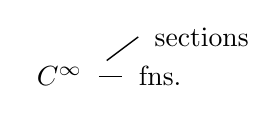
\begin{tikzpicture}[x=1mm,y=1mm,line width=.5pt]\node at (3,3) {$C^\infty$};\draw (8,3)--(11,3);\draw (9,5)--(13,8);\node[anchor=west,inner sep=0pt] at (13,3) {fns.};\node[anchor=west,inner sep=0pt] at (15,8) {sections};\end{tikzpicture}}
\begin{equation*}
\mathcal E(E_0)\qquad\mathcal E(E_1)
\end{equation*}
and morphisms
\begin{equation*}
\mathcal E(E_0)\overset{A}{\longrightarrow}\mathcal E(E_1)
\end{equation*}
([An entry is cancelled; below it, morph.]
$\forall$ given by diff. operators)
\Unclear{GELFAND-P000052}{morphism-cancellation}{a short densely overwritten entry}
Locally, $\mathcal E(E_0)|_U$ --- smooth vector fns.
\SourceFigure{GELFAND-P000052}{local-matrix-diagram}{Two local entries; in the first, the lower restriction sign is densely overwritten: $U$ / $a$. Downward arrow from $C^{n_0}(U)$ to $C^{n_1}(U)$, with $A(U)$ at right.\par\smallskip\centering\color{black}\begin{tikzcd}[ampersand replacement=\&,row sep=large,column sep=small]
\mathcal E(E_0)|_U\approx{}\&C^{n_0}(U)\arrow[d,"A(U)"]\\
\mathcal E(E_1)|_U\approx{}\&C^{n_1}(U)
\end{tikzcd}}
diff. oper. --- a matrix. Symbol --- princ. part of the matrix.
\uuline{Locally} $\sigma(A)(x,\xi)$ --- princ. part of the char. matrix.
\Unclear{GELFAND-P000052}{symbol-argument}{The second argument of $\sigma(A)$ is densely overwritten; forms $\xi$ / $\zeta$ / $D$ are visible.}
(Select terms of highest degree
Formalize.
Tang. bundle --- vect. $F$
\SourceFigure{GELFAND-P000052}{tangent-bundle-diagram}{Diagram with $X$, $T(X)$, $\pi$, $\pi^*E_0$, $\pi^*E_1$, $\sigma(A)$.\par\smallskip\centering\color{black}\begin{tikzcd}[ampersand replacement=\&]
\&X\&\\
\&T(X)\arrow[u,"\pi"]\&\\
\pi^*E_0\arrow[ur]\arrow[rr,"\sigma(A)"']\&\&\pi^*E_1\arrow[ul]
\end{tikzcd}}
$A$ ellipt. if $\sigma(A)$ is a monomorphism
(see Schwartz)
\underline{Example.}
\SourceFigure{GELFAND-P000052}{trivial-bundle-example}{At $E_0$, a leftward arrow; below $E_0$, fns.\par\smallskip\centering\color{black}$\underset{\text{fns.}}{E_0}\longleftarrow X\times\mathbf R^1\longrightarrow X$}
\begin{equation*}
\mathcal E(E_0)=C(X)\qquad C^\infty\text{ --- fns. on }X
\end{equation*}

\Needspace{5\baselineskip}
\SourcePage{GELFAND-P000053}{38}
\SourceFigure{GELFAND-P000053}{exterior-derivative-label}{Below $d$, ext. diff.\par\smallskip\centering\color{black}$C(X)\xrightarrow[\substack{\text{ext.}\\\text{diff.}}]{d}C^1(X)$}
Loc. $f(x)\longrightarrow\operatorname{grad}f(x)$
\underline{symbol} --- mult. by the vector $\xi\in T(X)$
This is an example of an overdet. elliptic system.
\begin{equation*}
f(x)\overset d{\longrightarrow}\sum\frac{\partial f}{\partial x_i}\,dx_i
\end{equation*}
\begin{equation*}
f(x)\longrightarrow
\begin{pmatrix}\dfrac\partial{\partial x_1}\\\vdots\\\dfrac\partial{\partial x_n}\end{pmatrix}f(x)
\end{equation*}
\begin{equation*}
E_0=X\times\mathbf R\longrightarrow X\qquad
E_1:\ \Lambda T(X)\longrightarrow X
\end{equation*}
\Unclear{GELFAND-P000053}{form-bundle}{At the end of the first line, a heavily overwritten $X$. After $E_1$, a dense cancellation before the colon; the sign before $T(X)$ resembles $\Lambda$ / $\wedge$. No clear star at $T$ is visible.}
[At right:] diff. forms --- sections of such a bundle.
\underline{Result.}
\begin{equation*}
\mathcal E(E_0)\overset A{\longrightarrow}\mathcal E(E_1)
\end{equation*}
Take
\begin{equation*}
0\longrightarrow\ker A\longrightarrow\mathcal E(E_0)
\overset A{\longrightarrow}\mathcal E(E_1)
\end{equation*}
If $A$ is ellipt., then
\begin{equation*}
\dim H^i(X,\ker A)<\infty
\end{equation*}
\underline{special cases.}
1°. Let $A$ be ellipt. in Petrovskii's sense.
\begin{equation*}
\mathcal E(\mathbf R^n)\overset A{\longrightarrow}\mathcal E(\mathbf R^n)
\end{equation*}
Then the space of glob. solutions is finite-dimensional
\begin{equation*}
H^0\quad\text{--- finite:}\qquad H^1\quad\text{--- defect. (fin. defect)}
\end{equation*}
\begin{equation*}
H^1(X,\ker A)
\end{equation*}
2°. Ext. diff. oper.
\SourceFigure{GELFAND-P000053}{constant-sheaf-label}{Below $\ker d$, const. sheaf.\par\smallskip\centering\color{black}$\dim H^i(X,\underset{\text{const. sheaf}}{\ker d})\quad\text{--- Betti numbers.}$}
3°. Compl. an. Cartan--Serre--Kodaira theorem

\Needspace{5\baselineskip}
\SourcePage{GELFAND-P000054}{unlabelled}
\SourceFigure{GELFAND-P000054}{heading-overwriting}{Several letters in the heading are densely overwritten.\par\smallskip\centering\color{black}\underline{Proof.}}
\SourceFigure{GELFAND-P000054}{bibliography-insertion}{Mac Lane inserted below within the parenthesis; two closing parentheses at right.\par\smallskip\centering\color{black}\begin{tabular}{@{}p{.44\linewidth}@{\quad}p{.44\linewidth}@{}}(read Godement,&Cartan and Eilenberg)\\\quad Mac Lane)&\end{tabular}}
$\mathcal P\longrightarrow$ a sheaf. How to compute homology.
\begin{equation*}
0\longrightarrow\mathcal P\longrightarrow\mathcal P_0\longrightarrow\mathcal P_1\longrightarrow\cdots.
\end{equation*}
a fine resolution.
\par\noindent\begin{minipage}{\linewidth}
\begin{equation*}
0\longrightarrow\underset{\underline{\text{sections}}}{\mathcal P_0(X)}\overset{d_0}{\longrightarrow}\mathcal P_1(X)\overset{d_1}{\longrightarrow}\cdots
\end{equation*}
\Unclear{GELFAND-P000054}{differential-labels}{The arrow subscripts are heavily inked. The visible candidates are $0$ and $1$.}
\end{minipage}\par
\SourceFigure{GELFAND-P000054}{sections-label}{Below $\mathcal P_0(X)$, sections underlined.\par\smallskip\centering\color{black}$\underset{\underline{\text{sections}}}{\mathcal P_0(X)}$}
\begin{equation*}
H^1(X,\mathcal P)=\ker d_1/\operatorname{Im}d_0
\end{equation*}
\begin{equation*}
0\longrightarrow\ker A\longrightarrow\mathcal E(\mathbf R^n)\overset A{\longrightarrow}\mathcal E(\mathbf R^n)
\end{equation*}
this is a fine resolution.
$H^1$ --- quotient.
The others, for an oper. ellipt. in Petrov.'s sense, 0.
\SourceFigure{GELFAND-P000054}{euler-characteristic-frame}{At left, Idea underlined, beside Of proof with a wavy underline; downward arrow and a long oval/stepped line.\par\smallskip\centering\color{black}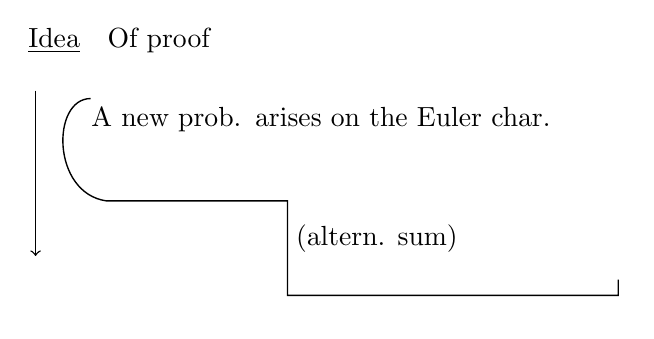
\begin{tikzpicture}[x=1mm,y=-1mm,line width=.5pt]
\path[use as bounding box](0,0)rectangle(76,36);
\node[anchor=north west,inner sep=0]at(0,0){\underline{Idea}\quad\uwave{Of proof}};
\draw[->](1,8)--(1,29);
\node[anchor=north west,align=left,text width=63mm,inner sep=0]at(8,10){A new prob. arises on the Euler char.};
\node[anchor=north west,inner sep=0]at(34,25){(altern. sum)};
\draw(8,9)..controls(3,9)and(3,21)..(10,22)--(33,22)--(33,34)--(75,34)--(75,32);
\end{tikzpicture}}
2 methods.
\SourceFigure{GELFAND-P000054}{schwarz-connector}{Kodaira and the line Reduc. to the Schwarz lemma have wavy lines; arrow to the following line.\par\smallskip\centering\color{black}\begin{minipage}{\linewidth}\uwave{Kodaira:} space of solns. of an ellipt. eqn.\par \uwave{Reduc. to the Schwarz lemma,}\par\begin{tikzpicture}[x=1mm,y=-1mm]\path[use as bounding box](0,0)rectangle(12,8);\draw[->](10,0)--(3,7);\end{tikzpicture}\par does not carry over to higher hom. (no theorems $A$ and $B$)\end{minipage}}
\Unclear{GELFAND-P000054}{second-method}{Another method: introd. top. / thin. and вп.-непр. ident. oper. [введ. / ввод. топ. / тон.; the initial abbreviations are not established.]}
Resolution from Ban. spaces.
\underline{Banach sheaf.}
Sheaf $\mathcal P$: $U\longrightarrow\mathcal P(U)$ (presheaf)
of Fréchet type $\mathcal P(U)$ --- $F$-spaces, and the restr. maps are cont.
A series of new sheaves
\begin{equation*}
C^{p,r}(\mathcal P)
\end{equation*}
\SourceFigure{GELFAND-P000054}{cochain-arrow}{The arrow from $U$ has a wavy beginning and an arrowhead at right.\par\smallskip\centering\(U\mathrel{\tikz[baseline=-.5ex,x=1mm,y=1mm]{\draw[->,line width=.5pt](0,0)--(1,.5)--(2,-.5)--(3,.5)--(4,-.5)--(5,.5)--(6,0)--(16,0);}}C_U^{p,r}(\mathcal P(U))\)}
Vect.-valued diff. forms of degree $p$, smoothness $r$
The sheaf extends, but with no add. assumpt., it does not extend.

\Needspace{5\baselineskip}
\SourcePage{GELFAND-P000055}{39}
For $\mathcal P=\mathcal E(E)$ Sheaf --- a Fréchet space.
de Rham resolution.
\begin{equation*}
0\longrightarrow\mathbf R\overset d{\longrightarrow}C^{0,r}
\overset d{\longrightarrow}C^{1,r}\overset d{\longrightarrow}\cdots.
\end{equation*}
\SourceFigure{GELFAND-P000055}{de-rham-bracket}{Below the sequence, a long bracket.\par\smallskip\centering\color{black}\begin{tikzpicture}[x=1mm,y=-1mm,line width=.5pt]
\path[use as bounding box](0,0)rectangle(72,7);
\draw(1,0)..controls(1,3)and(1,4)..(3,4)--(70,4);
\end{tikzpicture}}
[Below it, a sign is cancelled.]
\Unclear{GELFAND-P000055}{de-rham-cancellation}{a short densely cancelled sign}
Coeffs. --- maps of $U$ into diff. forms.
coeffs. --- smooth maps $U\longrightarrow\mathcal P(U)$
$r$ --- smoothness exponent.
Passing to the sheaf adds no new sections (but not in the gen. case, under add. assump.)
Of the type of the de Rham resolution
\begin{equation*}
0\longrightarrow\mathcal P\longrightarrow\widehat C^{p,r}(\mathcal P)
\overset d{\longrightarrow}\widehat C^{1,r}(\mathcal P)\longrightarrow\cdots.
\end{equation*}
adjusted because of the order of smoothness
Banach spaces result.
$H^i(X,\mathcal P)$ new [нов.; provisional] topol.
\Unclear{GELFAND-P000055}{cohomology-topology}{The heavily overwritten abbreviation before топ. [topol.] resembles нов. [new]; над. is another possibility.}
It does not depend on the choice of resolutions.
\begin{equation*}
H^i(X,\mathcal P)^{(r)}\longrightarrow H^i(X,\mathcal P)^{(r-1)}
\end{equation*}
take the same Fréchet spaces (isomorphism)
It is compl. cont. by the embedding theorem

\underline{Gelfand.} Problem: $X$ --- comp. with a sheaf of lin. top. spaces on it.
\underline{Ex.} $X$ --- a point. Just a space.
Diff. oper. --- endom. into itself.
\Unclear{GELFAND-P000055}{endomorphism}{The abbreviation before “into itself” is heavily overwritten and resembles endom.; below it “of the sheaf” is inserted and underlined.\par\smallskip\centering\color{black}$\underset{\underline{\text{of the sheaf}}}{\text{endom.}}$}
[At right:] (fibres preserved.)
When it is of finite index.
$X$ --- 1 point. $E+$ compl. cont. Riesz theorem.
Then one can \underline{consider} \underline{operators} ellipt. of order $\infty$.
\underline{Dynin.}
Hypoellipt. of the operator is needed. in the resolution, always the same sheaf $\ker A$
Merely cont. coeffs., will it be of finite index?
\underline{Next time.} Adams (Novikov), Berezin ($P$ and $Q$)
\Unclear{GELFAND-P000055}{next-talk}{The last letter in the parenthesis resembles $Q$ with a lower right stroke; $O$ remains possible.}

\Needspace{5\baselineskip}
\SourcePage{GELFAND-P000056}{unlabelled}
\SourceFigure{GELFAND-P000056}{date-and-speaker}{Date in a frame open at the top; below it, Adams; Novikov underlined twice.\par\smallskip\centering\color{black}\begin{tikzpicture}[x=1mm,y=-1mm,line width=.5pt]
\path[use as bounding box](0,0)rectangle(76,22);
\draw(1,1)--(1,12)--(24,12)--(24,1);
\node[anchor=north west,inner sep=0]at(2,2){$22/\mathrm{II}.$};
\node[anchor=north west,inner sep=0]at(6,14){\underline{Adams.}};
\node[anchor=north west,inner sep=0]at(30,3){\uuline{Novikov} S.P.};
\end{tikzpicture}}
$S^n$ how many lin. indep. vect. fields? (cont. f.)
\SourceFigure{GELFAND-P000056}{question-annotation}{Below how many, $\nu(n)$.\par\smallskip\centering\color{black}$\underset{\nu(n)}{\text{how many}}$}
\underline{Triv. facts.}
Exist on odd-dim. sph. ($\nu(n)\geq1$)
on even-dim. sph., none ($\nu(n)=0$)
\begin{equation*}
\sum\text{ind. of sing.}=\text{Euler char.}
\end{equation*}
$M^n$ --- $n$-dim. м-о. / м-ф.
\Unclear{GELFAND-P000056}{vector-graph}{м-о. / м-ф. [the last sign of the abbreviation is dense].\par\smallskip\centering\color{black}$\begin{gathered}\underset{\text{graph.}}{(m,\varphi(m))\subset(M^n,\mathbf R^n)}\\\underset{\text{vector field}}{(m,T_m)}\end{gathered}$}
$(m,0)$ --- canon.
Its intersection index is the index of the singularity.
\Unclear{GELFAND-P000056}{zero-section}{Below the line, a wavy bracket to $c(m,0)$ / $\varepsilon(m,0)$.\par\smallskip\centering\color{black}\begin{tikzpicture}[x=1mm,y=-1mm,line width=.5pt]
\path[use as bounding box](0,0)rectangle(72,16);
\draw(1,3)..controls(6,0)and(10,6)..(16,3)..controls(22,0)and(26,6)..(32,3)..controls(38,0)and(42,6)..(48,3)..controls(54,0)and(58,6)..(64,3);
\node[anchor=north,inner sep=0]at(58,7){$c(m,0)$};
\end{tikzpicture}}
(Here only 1 and $-1$, but degree $n$).
$E=2$, so there are no fields.
2) $S^3$ and $S^7$ paralleliz.
\Unclear{GELFAND-P000056}{sphere-three-seven}{Before the following equalities, a short cancelled entry; the upper sign of the second sphere resembles $7$ / an asterisk.}
$\nu(3)=3$, $\nu(7)=7$
3) $\nu(2n-1)\geq1$ ($S^{2n-1}$)
\par\noindent\begin{minipage}{\linewidth}
4) If on $S^{2m-1}$ there are $k$ indep. fields ($\nu(2m-1)\geq k$), then
on $S^{2pn-1}$, $\nu_{2pn-1}\geq k$
\Unclear{GELFAND-P000056}{sphere-continuation}{After $p$ the one-humped sign resembles $n$ more than the $m$ on the preceding line. Readings $2pn-1$ / $2pm-1$.}
\end{minipage}\par
In short
\begin{equation*}
S^{m-1},\quad\nu_m\geq k\quad\Longrightarrow\quad S^{pm-1},\quad\nu_{pm-1}\geq k
\end{equation*}
\SourceFigure{GELFAND-P000056}{coordinate-space-labels}{Below the sum, $\mathbf R^m$; at right, $\mathbf R^{pm}$.\par\smallskip\centering\color{black}$\underset{\mathbf R^m}{\sum_{i=1}^m x_i^2=1}\qquad\mathbf R^{pm}$}
\par\noindent\begin{minipage}{\linewidth}
Coords. $p$ groups of $m$ each
\Unclear{GELFAND-P000056}{block-indices}{$x_i^{(j)}$ / $y_i^{(j)}$ [first symbol overwritten], $i=1,\ldots,m$, $j=1,\ldots,p$.}
\end{minipage}\par
let $p=2$.
\SourceFigure{GELFAND-P000056}{two-block-labels}{Below each sum, $\mathbf R^m$. Asterisk after 1; no footnote on the frame.\par\smallskip\centering\color{black}$\underset{\mathbf R^m}{\sum y_i^2}+\underset{\mathbf R^m}{\sum z_i^2}=1^*$}
\begin{equation*}
v(x)\text{ in }\mathbf R^m,\qquad v(x)\perp x\qquad(\text{field on }S^{m-1})
\end{equation*}
\Unclear{GELFAND-P000056}{bottom-vector-sign}{The initial letter in $v(x)$ resembles Latin $v$ / $\nu$; no separate quantifier sign is established.}

\Needspace{5\baselineskip}
\SourcePage{GELFAND-P000057}{40}
Put
\begin{equation*}
\widetilde v(y,z)=\left(\|y\|v\left(\frac y{\|y\|}\right),\ \|z\|v\left(\frac z{\|z\|}\right)\right)
\end{equation*}
$\|y\|$ to cope with $y=0$, all in the 2nd comp.,
of $\operatorname{mod}=1$, and $\perp(y,z)$
Indep. fields are obtained from indep. fields.
Thus Hopf fields are obt.
(On the right one can write other fields)
can stabilize the problem: incr. dim.
Was known to the classical authors (hard to construct.
\SourceFigure{GELFAND-P000057}{classification-oval}{At left, $S^{m-1}$ in an oval. The upper stroke overlaps Was. Arrow down.\par\smallskip\centering\color{black}\begin{tikzpicture}[x=1mm,y=-1mm,line width=.5pt]
\path[use as bounding box](0,0)rectangle(35,32);
\draw(14,7)ellipse(12mm and 6mm);
\node[inner sep=0]at(14,7){$S^{m-1}$};
\draw[->](21,12)..controls(25,19)and(26,23)..(28,30);
\end{tikzpicture}}
\begin{equation*}
m=2^b(2a+1)\qquad b=c+4d\qquad0\leq e\leq3,
\end{equation*}
\Unclear{GELFAND-P000057}{range-letter}{In the bounds $0\leq e\leq3$, the middle letter resembles $e$ / $c$.}
\par\noindent\begin{minipage}{\linewidth}
then the known number of fields
\SourceFigure{GELFAND-P000057}{field-count-frame}{Frame open at the top; the exponent resembles $e$ / $c$.\par\smallskip\centering\color{black}\begin{tikzpicture}[x=1mm,y=-1mm,line width=.5pt]
\path[use as bounding box](0,0)rectangle(40,12);
\node[inner sep=0]at(20,5){$2^e+8d-1$};
\draw(1,1)--(1,10)--(39,10)--(39,1);
\end{tikzpicture}}
\end{minipage}\par
\begin{equation*}
\nu_{m-1}\geq2^c+8d-1
\end{equation*}
In cases 3, 7 gives max.
$b=0$ (even --- triv.).
$b=1,2,3$, [a sign is overwritten], simple, but req. methods of alg. top.
\Unclear{GELFAND-P000057}{low-exponent-sign}{densely overwritten sign / downward arrow}
$b\leq12$ Toda, but $m$ of order 3000
Adams proved this in all dimensions.
\SourceFigure{GELFAND-P000057}{adams-emphasis}{Two wavy underlines.\par\smallskip\centering\color{black}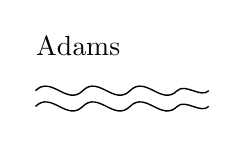
\begin{tikzpicture}[x=1mm,y=-1mm,line width=.5pt]
\path[use as bounding box](0,0)rectangle(24,12);
\node[anchor=north west,inner sep=0]at(1,1){Adams};
\draw(1,8)..controls(3,6)and(5,10)..(7,8)..controls(9,6)and(11,10)..(13,8)..controls(15,6)and(17,10)..(19,8)..controls(20,7)and(22,9)..(23,8);
\draw(1,10)..controls(3,8)and(5,12)..(7,10)..controls(9,8)and(11,12)..(13,10)..controls(15,8)and(17,12)..(19,10)..controls(20,9)and(22,11)..(23,10);
\end{tikzpicture}}
$\ast$ The reduct. part belongs to Atiyah and Toda. This leads to a problem on homot. gr. of spheres.
finally
\begin{equation*}
\nu_{m-1}=2^c+8d-1
\end{equation*}
The odd factor plays no role.
\par\noindent\begin{minipage}{\linewidth}
Here one assertion. $m\uparrow$ by a factor of 6, then the number of fields incr. by 8
\EvidenceBlock{GELFAND-P000057}{growth-factor}{The factor is written as $6$.}{Manuscript notation.}
\end{minipage}\par
$(d+1)$ this is seen from the constr. in Bott periodicity.
For the first ones all is known.
\Unclear{GELFAND-P000057}{bott-comment}{After $1$ are a short stroke and an x-shaped sign. The proposed reading is 1-х [the first ones].}
2 parall. sph., then Bott periodicity
\SourceFigure{GELFAND-P000057}{homotopy-table}{Asterisks below 1, 2, 4, 8.\par\smallskip\centering\color{black}$\pi_i(BO).\qquad
\begin{array}{cccccccc}
i=1&2&3&4&5&6&7&8\\
*&*& &*& & & &*
\end{array}$}
\underline{where} $\underline{\pi_i}$ of Grassm. mfld. is nontriv.
$\mathbf RP^k$ --- project. space
Consid. \Unclear{GELFAND-P000057}{k-theory-bottom}{In the lower entry $f(k)$ is raised relative to $2$. Readings $2^{f(k)}$ / $2f(k)$. The small upper sign on $\widetilde K$ resembles $0$. From the second summand a bracket to the lower entry.\par\smallskip\centering\color{black}\begin{tikzpicture}[x=1mm,y=-1mm,line width=.5pt]
\path[use as bounding box](0,0)rectangle(75,30);
\node[anchor=north west,inner sep=0]at(1,1){$K_{\mathbf R}(\mathbf RP^k)=\mathbf Z+\widetilde K_{\mathbf R}^{0}$};
\draw(43,10)..controls(45,15)and(49,15)..(53,14)..controls(57,13)and(60,12)..(62,12)..controls(63,11)and(64,14)..(65,12)..controls(66,11)and(67,13)..(68,12);
\node[anchor=north west,inner sep=0]at(45,18){$\widetilde K_{\mathbf R}=\mathbf Z_{2^{f(k)}}$};
\end{tikzpicture}}
$K$-functor, see “Матем.” [Math.] Atiyah and Hirzebruch

\Needspace{5\baselineskip}
\SourcePage{GELFAND-P000058}{unlabelled}
Elem. of $K$ --- real vect. bundle, but with an equiv. relation.
Add. --- direct $\Sigma$. Mult. --- tensor prod. of 2 vect. bund.
1 elem. in $K$, if
\begin{equation*}
O_{N_1}\oplus\eta=O_{N_2}\oplus\zeta\quad\Longrightarrow\quad\eta\overset K\sim\xi
\end{equation*}
\Unclear{GELFAND-P000058}{stable-equivalence}{After the second sum the sign resembles $\zeta$; after the equivalence it resembles $\xi$ / $\zeta$. The initial oval permits $O$ / $0$.}
\begin{equation*}
\underline{O_N=X\times\mathbf R^N}
\end{equation*}
[At right:] (can twist it)
Bund. up to equiv. --- element of the $K$-funct.
Coll. --- $K$-functor. Can add, mult.!
Triv. bund. ($\Sigma$ of tang. and norm. --- triv., there is an inverse elem.)
To each space assigns a ring)
\underline{Over the sphere} $K$-functor
\begin{equation*}
K_{\mathbf R}(S^i)=\pi_i(BO)
\end{equation*}
(how many homot. maps to Grassm. mfld.)
\SourceFigure{GELFAND-P000058}{grassmann-insertion}{Above large, the insertion Grassm. mfld.\par\smallskip\centering\color{black}$K$-funct. of sph. --- bund. of $\overset{\text{Grassm. mfld.}}{\text{large}}$ dim.}
$BO$ --- Grassm. mfld. --- $n$-dim. lin. in $N$-dim. sp.
($n$ and $N$ large)
\Unclear{GELFAND-P000058}{stabilization-tail}{Below, everything stabilizes; the long tail of the parenthesis overlaps the end of the word.\par\smallskip\centering\color{black}
\begin{tikzpicture}[x=1mm,y=-1mm,line width=.5pt]
\path[use as bounding box](0,0)rectangle(65,12);
\node[anchor=north west,inner sep=0,text width=60mm]at(1,2){everything stabilizes};
\draw(60,.5)..controls(61,3)and(60,4)..(55,5);
\end{tikzpicture}}
\par\noindent\begin{minipage}{\linewidth}
Vect. bund. with given base $\longleftarrow$ evident $\pi_i$.
\EvidenceBlock{GELFAND-P000058}{classifying-map}{The abbreviation before $\pi_i$ reads очев. [evident].}{Manuscript notation.}
\end{minipage}\par
To the mfld. corresp. tang. spher. maps.
To the normal sheaf --- norm. spher. map. Next an artificial device.
$\mathbf RP^k$ subdiv. into cells (1 in each dim.)
All vect. bund. over $\mathbf RP^k$ are constr. thus.
\begin{equation*}
\sigma^i\quad\text{--- $i$-dim. cell of }\mathbf RP^k
\end{equation*}
\Unclear{GELFAND-P000058}{cell-bundle}{After $\sigma^i$ a short entry densely cancelled; below it, $\mathbf RP^i\longrightarrow\mathbf RP^{i-1}$. Above the first $\mathbf RP^i$ a small unidentified sign.\par\smallskip\centering\color{black}$\mathbf RP^i\longrightarrow\mathbf RP^{i-1}$}
consid.
\Unclear{GELFAND-P000058}{quotient-diagram}{Before $S^i$ a dense short sign, its reading not established. Below, $\mathbf RP^k/\mathbf RP^{i-1}$ with a curved arrow.\par\smallskip\centering\color{black}\begin{tikzpicture}[x=1mm,y=-1mm,line width=.5pt]
\path[use as bounding box](0,0)rectangle(69,44);
\node[anchor=north west,inner sep=0]at(1,1){$S^i=\mathbf RP^i/\mathbf RP^{i-1}$};
\node[anchor=north west,inner sep=0]at(13,32){$\mathbf RP^k/\mathbf RP^{i-1}$};
\draw[->](16,29)..controls(14,17)and(23,14)..(24,27);
\end{tikzpicture}}
All bund. are obtained thus.
Bund. $S^i\longrightarrow$ bund. over $\mathbf RP^i\longrightarrow$
\Incomplete{GELFAND-P000058}{bottom-continuation}{The arrow in the bottom line reaches the right edge; the next object is not visible in this frame.}

\Needspace{5\baselineskip}
\SourcePage{GELFAND-P000059}{41}
$\longrightarrow$ bund. on $\mathbf RP^k$.
$f(k)$ --- number of asterisks to the left of $k$
$\mathbf Z$ --- invar. --- dimension
Crit. points appear on cycles
\par\noindent\begin{minipage}{\linewidth}
\begin{equation*}
\mathbf Z_{2^{f(k)}}\qquad\text{cyclic gr. of order }f(k)
\end{equation*}
\Unclear{GELFAND-P000059}{cyclic-order}{The index on $\mathbf Z$ permits $2^{f(k)}$ / $2f(k)$; the order caption visibly has $f(k)$, without a separate $2$.}
\end{minipage}\par
[At left an entry is cancelled.]
\Unclear{GELFAND-P000059}{upper-cancellation}{short dense cancellation}
\par\noindent\begin{minipage}{\linewidth}
\begin{equation*}
\mathbf RP^k\in\mathbf RP^{k+1}
\end{equation*}
\EvidenceBlock{GELFAND-P000059}{projective-inclusion}{The sign has the middle stroke of $\in$. A separate $\subset$ appears lower on the page.}{Manuscript sign.}
\end{minipage}\par
there is a norm. sheaf --- Möbius strip
(this is a generator) of the group
it must be added to itself $2^{f(k)}$ times
\SourceFigure{GELFAND-P000059}{normal-bundle-diagram}{At left an almost horizontal line; five transverse arrows: two on the left down, the next three up. Two rightward arrows above the line, short on the left, long on the right. Below, an open oval arc with a gap at the lower right; its left end rises to the line and has an arrow, the right end is faint. No letter labels.\par\smallskip\centering\color{black}\begin{tikzpicture}[x=1mm,y=-1mm,line width=.5pt]
\path[use as bounding box](0,0)rectangle(73,30);
\draw(7,10)--(16,10);\draw(19,10)--(69,10);
\draw[->](17,6)--(16,15);\draw[->](22,6)--(22,15);
\draw[->](31,14)--(31,6);\draw[->](40,14)--(40,6);\draw[->](51,14)--(51,6);
\draw[->](5,4)--(14,4);\draw[->](51,4)--(69,4);
\draw[->](33,27)..controls(1,26)and(0,16)..(5,12);
\draw(39,27)..controls(43,27)and(48,26)..(54,25);
\draw(62,22)--(67,18);\draw(69,13)--(70,14);
\end{tikzpicture}}
\begin{align*}
\underline{\nu^2=1}\qquad&\lambda=\nu-1\\
\lambda^2&=1+1-2\nu\\
\lambda^2&=2(1-\nu)
\end{align*}
\Unclear{GELFAND-P000059}{lambda-symbols}{The narrow sign in $\nu$ resembles $\nu$ / $v$ / $V$; some equality signs are overwritten. The last line is in a rounded frame open at the top.\par\smallskip\centering\color{black}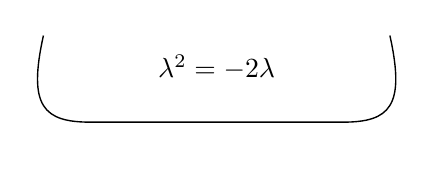
\begin{tikzpicture}[x=1mm,y=-1mm,line width=.5pt]
\path[use as bounding box](0,0)rectangle(48,15);
\node[inner sep=0]at(24,5){$\lambda^2=-2\lambda$};
\draw(2,1)..controls(0,10)and(2,12)..(8,12)--(40,12)..controls(46,12)and(48,10)..(46,1);
\end{tikzpicture}}
mult. structure.
[A line is cancelled.]
\Unclear{GELFAND-P000059}{lower-cancellation}{Long, densely crossed-out line on the left below the formulas}
There is
\SourceFigure{GELFAND-P000059}{inclusion-bars}{Above the right side are two horizontal strokes of different lengths with a dot between them.\par\smallskip\centering\color{black}\begin{tikzpicture}[x=1mm,y=-1mm,line width=.5pt]
\path[use as bounding box](0,0)rectangle(66,18);
\node[anchor=north west,inner sep=0]at(1,5){$\mathbf RP^{n-1}\subset O_n$};
\draw(49,3)--(54,3);\draw(58,2)--(65,2);\fill(56,2.7)circle(.3mm);
\end{tikzpicture}}
\par\noindent\begin{minipage}{\linewidth}
$S^n$ is assigned to the hyperpl. of the equator $\longrightarrow$ into the orthog. group.
Tang. sheaf --- map.
\Unclear{GELFAND-P000059}{sphere-map-insertion}{Above the arrow, a tight insertion $\mathbf RP^{n-1}$ / $\mathbf RP^n$ with an additional slanted arrow pointing to $O_n$; some signs are dense.\par\smallskip\centering\color{black}\begin{tikzpicture}[x=1mm,y=-1mm,line width=.5pt]
\path[use as bounding box](0,0)rectangle(65,24);
\node[inner sep=0]at(8,16){$S^{n-1}$};
\node[inner sep=0]at(53,16){$O_n$};
\node[inner sep=0]at(31,5){$\mathbf RP^{n-1}$};
\draw[->](20,16)--(43,16);\draw[->](42,8)--(48,13);
\end{tikzpicture}}
\end{minipage}\par
At symmetric points, the same.
it is \uuline{2-sheeted}
(Gluing on the equator)
rotation about it
\Unclear{GELFAND-P000059}{reflection-arrow}{From the parenthesis about reflection an arrow down to $O(n)$; before $O(n)$ a black overwritten stroke, reading not established.\par\smallskip\centering\color{black}\begin{tikzpicture}[x=1mm,y=-1mm,line width=.5pt]
\path[use as bounding box](0,0)rectangle(73,27);
\node[anchor=north west,inner sep=0,text width=68mm]at(1,1){(reflection about it)};
\draw[->](25,12)--(22,18);
\node[anchor=north west,inner sep=0]at(20,20){$O(n)$};
\end{tikzpicture}}
axes of proj. space.
\Unclear{GELFAND-P000059}{axis-name}{Albert Solom. / Soln.}
Schwarz.
\SourceFigure{GELFAND-P000059}{axis-diagram}{Slanted line with a point and the label axis in $\mathbf R^n$.\par\smallskip\centering\color{black}\begin{tikzpicture}[x=1mm,y=-1mm,line width=.5pt]
\path[use as bounding box](0,0)rectangle(69,34);
\draw(5,32)--(24,1);\fill(15,16)circle(.7mm);
\node[anchor=north west,inner sep=0]at(27,2){axis in $\mathbf R^n$};
\end{tikzpicture}}
\par\noindent\begin{minipage}{\linewidth}
\begin{equation*}
\mathbf RP^{n-1}/\mathbf RP^{n-k-2}\longrightarrow O_n/O_{n-k-1}
\end{equation*}
\Unclear{GELFAND-P000059}{quotient-map}{In the lower left exponent, $n-k-2$ / $n-n-2$; the arrow between the quotients is densely overwritten.}
\end{minipage}\par
in fact an embedding.

\Needspace{5\baselineskip}
\SourcePage{GELFAND-P000060}{unlabelled}
$1/\overline{\underline{\mathrm{III}}}$\par
\uwave{V.P. Palamodov.}
$\mathcal P$ --- ring of polyn. in $\mathbf C^n$,
$\mathcal J\subset\mathcal P$ --- ideal, primary,
$P_1,\ldots,P_s$ --- gener.
\par\noindent\begin{minipage}{\linewidth}
$\mathcal H$ --- ring of entire funct. [a sign is cancelled] of a conv. region
\Unclear{GELFAND-P000060}{whole-functions-cancellation}{after funct. a short sign is densely crossed out}
\end{minipage}\par
$\mathcal H/\mathcal J\mathcal H$ is described thus
\par\noindent\begin{minipage}{\linewidth}
\begin{equation*}
\mathcal H\{\mathcal J\}=\{f|_N\quad f(z)=d(z,\mathcal D)F_\zeta(z)\}
\end{equation*}
\Unclear{GELFAND-P000060}{local-f-index}{The subscript on $F$ resembles $\zeta$ / $s$.}
\end{minipage}\par
\par\noindent\begin{minipage}{\linewidth}
\begin{equation*}
\mathcal H/\mathcal J\mathcal H\cong\mathcal H\{\mathcal J\}\quad^{\text{local part}}
\end{equation*}
\EvidenceBlock{GELFAND-P000060}{local-part}{The note “local part” is written above and to the right of the second formula.}{Position of the note.}
\end{minipage}\par
Kazhdan says that $\underset{\longrightarrow}{\text{this}}$ is \underline{obt.} algebraically.

$\bullet$ \underline{Gelfand.}
\uwave{Nelson's example.}
2 self-adj. operators $A$ and $B$.
what changes a self-adj. oper.? (not symm. closed)
[In the right margin:]
\par\noindent\begin{minipage}{\linewidth}
\begin{equation*}
i\frac d{dx},\qquad y(a)=y(b)
\end{equation*}
\Unclear{GELFAND-P000060}{boundary-margin}{Below is written “or also $=0$”; no argument precedes the equality sign.}
\end{minipage}\par
Essentially self-adj. $A$ (symm.), if
there are no vect. orthog. to all vect. of the form
\par\noindent\begin{minipage}{\linewidth}
\begin{equation*}
\overline z=Ax-ix,\qquad z=Ax+ix
\end{equation*}
\Unclear{GELFAND-P000060}{range-z-marks}{The first $z$ has a long upper bar. The upper stroke of the second may be part of the letter or a separate mark.}
\end{minipage}\par
\par\noindent\begin{minipage}{\linewidth}
(Then [an entry is cancelled] the same $\forall$ complex $\lambda$)
\Unclear{GELFAND-P000060}{criterion-cancellation}{short dense cancellation}
\end{minipage}\par
otherwise $Ax-ix$ are everywhere dense
$A-iE$ has inv. (in general?: if closed)
\par\noindent\begin{minipage}{\linewidth}
\begin{equation*}
\left(i\frac d{dx}\quad\text{[on / not] even analyt.}\quad
\begin{array}{ll}
f(a)=f(b)&\text{\uwave{essentially self-adj.}}\\
f(a)=f(b)=0&\text{only symm.}
\end{array}\right)
\end{equation*}
\Unclear{GELFAND-P000060}{differential-qualifier}{Before the conditions is written “[on / not] even analyt.”; the last letter of the first word is joined.}
\end{minipage}\par
$A$ and $B$ essentially self-adj.,
$\alpha A+\beta B$ essentially self-adj.,
$\alpha,\beta$ --- real.
\begin{equation*}
\forall f\in\text{domain of def.}\qquad ABf=BAf.
\end{equation*}
\Unclear{GELFAND-P000060}{domain-cancellation}{Above the domain of definition a short entry is densely overwritten; below it a curved stroke.\par\smallskip\centering\color{black}\begin{tikzpicture}[x=1mm,y=-1mm,line width=.5pt]
\path[use as bounding box](0,0)rectangle(32,9);
\draw(1,1)..controls(2,9)and(7,8)..(11,6)..controls(15,10)and(20,4)..(30,2);
\end{tikzpicture}}
Nevertheless $A$ and $B$ do not commute.
\SourceFigure{GELFAND-P000060}{example-emphasis}{At left Example. is crossed out and doubly underlined; to its right a double vertical stroke.\par\smallskip\centering\color{black}\begin{tikzpicture}[x=1mm,y=-1mm,line width=.5pt]
\path[use as bounding box](0,0)rectangle(48,25);
\node[anchor=north west,inner sep=0]at(1,2){\uuline{\sout{Example.}}};
\draw(39,2)--(39,24);\draw(41,2)--(41,24);
\end{tikzpicture}}
$A$ and $B$ comm., if reasonabl. funct. of them commute.
\par\noindent\begin{minipage}{\linewidth}
\begin{equation*}
\underset{\text{oper. bounded}}{(A-\lambda E)^{-1}}
\end{equation*}
\Unclear{GELFAND-P000060}{resolvent-understroke}{Below $\lambda E$ lower strokes; whether a separate underline or parts of letters is not established.}
\end{minipage}\par
\par\noindent\begin{minipage}{\linewidth}
Comm. [Cancelled: \textcolor{orange!65!black}{not...}] also with $B$ means that these oper. too comm.
\Unclear{GELFAND-P000060}{resolvent-cancellation}{The cancelled entry begins with a mark resembling не [not]; the remaining letters are obscured.}
\end{minipage}\par
\begin{equation*}
e^{iA}\quad\text{--- unit.}\qquad e^{iB}\quad\text{do not commute}
\end{equation*}
\par\noindent\begin{minipage}{\linewidth}
[An entry is cancelled; beside it $(\forall\text{ bounded oper.})$.]
\Unclear{GELFAND-P000060}{final-cancellation}{Short densely crossed-out entry}
\end{minipage}\par

\Needspace{5\baselineskip}
\par\noindent\begin{minipage}{\linewidth}
\SourcePage{GELFAND-P000061}{42}
\uuline{Nelson's example.}
\SourceFigure{GELFAND-P000061}{nelson-grid}{Square grid, heavy points and central hatching; labels $0,1,2,3$ below, $1,2,3$ at left and $2$ at right. Between $1$ and $2$ at left, a sign resembling $3$ with a heavily inked lower stroke; the central overlapping strokes and exact gluing are not established.\par\smallskip\centering\color{black}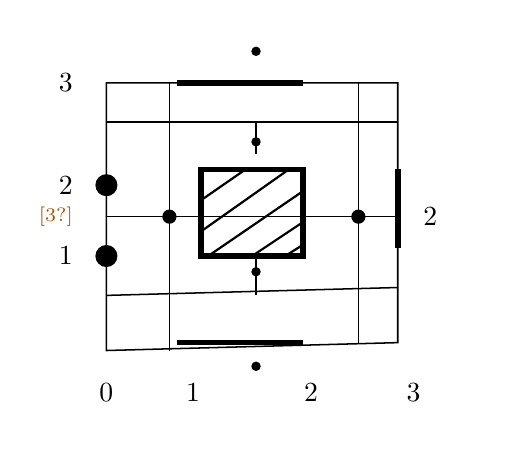
\begin{tikzpicture}[x=1mm,y=-1mm,line width=.55pt]
\path[use as bounding box](0,0)rectangle(58,53);
\draw(10,7)--(47,7)--(47,40)--(10,41)--cycle;
\draw(18,7)--(18,41);\draw(42,7)--(42,40);
\draw(10,12)--(47,12);\draw(10,24)--(47,24);\draw(10,34)--(47,33);
\draw(29,12)--(29,16);\draw(29,29)--(29,34);
\draw[line width=2pt](19,7)--(35,7);\draw[line width=2pt](19,40)--(35,40);
\draw[line width=2pt](47,18)--(47,28);
\fill(10,20)circle(1.4);\fill(10,29)circle(1.4);
\fill(18,24)circle(.9);\fill(42,24)circle(.9);
\fill(29,14.5)circle(.6);\fill(29,31)circle(.6);
\draw[line width=2.1pt](22,18)--(35,18)--(35,29)--(22,29)--cycle;
\begin{scope}\clip(22,18)rectangle(35,29);
\draw[line width=.8pt](19,24)--(32,15);\draw[line width=.8pt](19,28)--(36,16);
\draw[line width=.8pt](20,31)--(39,18);\draw[line width=.8pt](24,32)--(39,22);
\draw[line width=.8pt](28,32)--(39,25);\end{scope}
\node[anchor=east]at(7,7){$3$};\node[anchor=east]at(7,20){$2$};
\node[anchor=east]at(7,29){$1$};\node[anchor=east]at(7,24){\scriptsize\textcolor{orange!65!black}{[$3$?]}};
\node[anchor=north]at(10,44){$0$};\node[anchor=north]at(21,44){$1$};
\node[anchor=north]at(36,44){$2$};\node[anchor=north]at(49,44){$3$};
\node[anchor=west]at(49,24){$2$};\fill(29,3)circle(.6);\fill(29,43)circle(.6);
\end{tikzpicture}}
\end{minipage}\par
From the region between the squares, remove the heavy points
The segments are glued
each point is glued to the nearest boundary point along the horiz. or vert.
The corners are glued together. Obtain a surface of genus
\textcolor{orange!65!black}{$\underline{4}$}
with one removed point
\Unclear{GELFAND-P000061}{genus}{The numeral has an angular top and a broad foot. Prefer $4$; $1$ is also possible.}
\par\noindent\begin{minipage}{\linewidth}
\begin{equation*}
X=\frac{d}{dx},\qquad y=\frac{d}{dy}
\end{equation*}
\Unclear{GELFAND-P000061}{generator-symbol}{The second sign before the equality has the descender of $y$; the later entry is $iY$.}
\end{minipage}\par
$iX$, $iY$ --- formally self-adj.
They commute
But the corresp. oper. do not commute.
Remove measure-$0$ closed traject. hitting the vertices.
$e^X$ and $e^Y$ --- unit. oper. which do not commute.
\begin{equation*}
e^{\frac{d}{dx}}f(x)=f(x+1)
\end{equation*}
(Taylor formula)
Prove first for analytic funct., then for the whole Hilb.
space by a limiting passage (the oper. is unitary)
And it has to be moved.
\SourceFigure{GELFAND-P000061}{shift-square}{Square with a hole; hatching to the left of the hole and in the lower left region, two short strokes to its right. A slanted line runs from the lower left region down towards the caption. The boundaries of the overlapping strokes are not established.\par\smallskip\centering\color{black}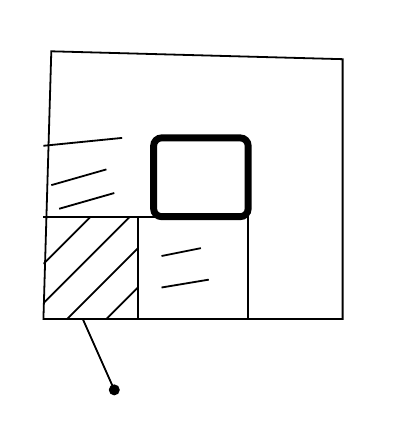
\begin{tikzpicture}[x=1mm,y=-1mm,line width=.65pt]
\path[use as bounding box](-2,-2)rectangle(44,47);
\draw(1,1)--(38,2)--(38,35)--(0,35)--cycle;
\draw(0,22)--(26,22)--(26,35);\draw(12,22)--(12,35);
\draw[line width=2.5pt,rounded corners=1mm](14,12)rectangle(26,22);
\draw(0,13)--(10,12);\draw(1,18)--(8,16);\draw(2,21)--(9,19);
\begin{scope}\clip(0,22)rectangle(12,35);
\draw(0,28)--(6,22);\draw(0,33)--(11,22);\draw(3,35)--(12,26);\draw(8,35)--(12,31);
\end{scope}
\draw(15,27)--(20,26);\draw(15,31)--(21,30);
\draw(5,35)--(9,44);\fill(9,44)circle(.7);
\end{tikzpicture}}
$e^Y$ --- region by $1$ upwards, $e^X$ will turn round
\begin{equation*}e^X\end{equation*}
funct. with \textcolor{orange!65!black}{compact. [компт.]} here.
\Unclear{GELFAND-P000061}{support-word}{compact. / comp. [компт. / комп.]}
Exclude a finite number of traject.
$e^{tX}$ --- shift along the traject. of oper. $X$
locally everywhere they commute
\par\noindent\begin{minipage}{\linewidth}
what will happen to [Inserted above: with] the Laplace oper.?
\EvidenceBlock{GELFAND-P000061}{laplace-overwrite}{The letter с [with] is above a caret.}{Manuscript insertion.}
\end{minipage}\par
deficiency index
\begin{gather*}
\Delta f=if\\
\underline{\Delta=X^2+Y^2}
\end{gather*}
(this follows from Nelson's theorem)
It is not self-adj. (has a $C^\infty$ solution, bound. cond., and at the point only $\int$ square.)
The shift oper. themselves are def. on $L^2$, and not on periodic funct.
\underline{3 def.}
$e^{itA}$:
\par\noindent\begin{minipage}{\linewidth}
\begin{align*}
1^\circ&=\int_{-\infty}^{+\infty}\frac{e^{it\lambda}}{iA-\lambda}\,d\lambda\\
2^\circ&=\int_{-\infty}^{+\infty}e^{it\lambda}\,dE_\lambda\\
3^\circ&:\quad \frac{df}{dt}=iAf
\end{align*}
\Unclear{GELFAND-P000061}{resolvent}{In the first entry the denominator is $iA-\lambda$; no separate factor before the integral is visible.}
\Unclear{GELFAND-P000061}{evolution-prefix}{Before the fraction in the third line, a short dark stroke; the exact reading is not established.}
\end{minipage}\par
$\underset{\text{sol.}}{U}_{t,0}f_0=f$ --- unit. oper.

\Needspace{5\baselineskip}
\SourcePage{GELFAND-P000062}{unlabelled}
\uwave{Sinai.} \uwave{Posit. in dyn. systems.} [Полож.]
For an ergod. dyn. syst.
[Crossed out: a short densely crossed-out entry; inserted above: with discr. spec.]
the spectrum is always simple
\Unclear{GELFAND-P000062}{cancelled-spectrum}{a short densely crossed-out entry}
$M$, $\mu$, $\{S_t\}$ --- one-param. gr. in $M$
In $\mathcal L^2_\mu$
a one-param. gr. of unit. oper.
\par\noindent\begin{minipage}{\linewidth}
\begin{equation*}
\underset{\tikz[baseline=-.5ex]{\draw[->] (0,1.7mm) .. controls (2mm,0) and (7mm,0) .. (9mm,1.7mm);}}{U_t}f(x)=f(S_t x)
\end{equation*}
\EvidenceBlock{GELFAND-P000062}{operator-curve}{Below $U_t$ is a curve with a pointed right end; “simple” belongs to the following line.}{Manuscript sign.}
\end{minipage}\par
In the ergod. case every eigenvalue is simple
\uwave{Lebesgue spectrum:}
$\forall f$
\begin{equation*}
(U_t f,f)=\int e^{it\lambda}p(\lambda)\,d\lambda
\end{equation*}
($p(\lambda)$ --- integr.)
(In general always $\int e^{it\lambda}\,d\mu$, here $\mu$ abs. cont.)
\uwave{Countably-mult. Leb. spec.}:
$\exists$ orthog. $f_1,f_2,\ldots$
\begin{equation*}
(U_t f_i,f_j)=0\qquad(i\neq j)
\end{equation*}
and generate everything.
In all known ex. the spectrum is countably-mult.
\underline{Ex.} \uwave{Transf. of the torus.}
\begin{equation*}
\begin{pmatrix}a&b\\c&d\end{pmatrix},
\qquad \det=1,\quad\text{integer}
\end{equation*}
\begin{gather*}
x\longrightarrow ax+by\\
y\longrightarrow cx+dy
\end{gather*}
Need to find autocorr. [авток.] Expand in a Fourier series and act.
\begin{gather*}
f(x,y)\longrightarrow f(ax+by,cx+dy)\\
e^{2\pi i(mx+ny)}
\longrightarrow e^{2\pi i((am+cn)x+(bm+dn)y)}
\end{gather*}
A matrix acts on the integer latt.
Need to take trajectories
\begin{equation*}
(m,n)\longrightarrow S(m,n)=(m',n')
\end{equation*}
The traject. is a hyperbola.
\SourceFigure{GELFAND-P000062}{hyperbola}{Above, two crossing strokes without explicit arrows. Below, an oblique line and two curved strokes; thickening at the crossing. The upper right end of the oblique line and the bottom end of the long curved stroke resemble arrows; the membership of the overlapping strokes is not established.\par\smallskip\centering\color{black}\begin{tikzpicture}[x=1mm,y=-1mm,line width=.6pt]
\path[use as bounding box](0,0)rectangle(43,23);
\draw(3,14)..controls(17,14)and(29,14)..(40,12);
\draw(16,2)--(18,21);
\end{tikzpicture}
\par\smallskip
\begin{tikzpicture}[x=1mm,y=-1mm,line width=.65pt]
\path[use as bounding box](0,0)rectangle(48,58);
\draw[->](3,52)--(44,15);
\draw[->](16,5)..controls(20,21)and(22,31)..(27,55);
\draw(21,2)..controls(22,15)and(25,33)..(35,24)..controls(37,22)and(38,20)..(39,18);
\draw[line width=1.7pt](22,29)--(24,34);
\end{tikzpicture}}
Real eigenvalues --- contraction along one axis
and expansion along the other ($\det=1$)
\par\noindent\begin{minipage}{\linewidth}
\begin{equation*}
S^k\left(\frac mn\right)\longrightarrow\lambda
\end{equation*}
($\lambda$ --- eigenvalue)
\Unclear{GELFAND-P000062}{frequency-limit}{A horizontal stroke separates $m$ from $n$. The arrow points to $\lambda$; no additional factor is visible.}
\end{minipage}\par
The waves become ever denser and direct.
Waves $\Longrightarrow$ towards an eigendir.
The space decomposes into a space of funct. with frequencies on
hyperbolas. On the $1$st hyperbola.
A sequence of orthog. vect., each passes to the next

\Needspace{5\baselineskip}
\SourcePage{GELFAND-P000063}{43}
\SourceFigure{GELFAND-P000063}{shift-points}{Above, a row of nine separate points.\par\smallskip\centering\color{black}\begin{tikzpicture}[x=1mm,y=1mm]
\path[use as bounding box](0,-2)rectangle(71,3);
\fill(2,0)circle(.45);\fill(10,.4)circle(.6);\fill(18.7,.3)circle(.55);
\fill(27.4,.1)circle(.5);\fill(34.7,.5)circle(.35);\fill(42.1,.6)circle(.35);
\fill(50.1,.3)circle(.4);\fill(55.5,.2)circle(.3);\fill(65.2,.5)circle(.35);
\end{tikzpicture}}
(shift by $1$ at the integer pts.)
cont. Lebesgue spectrum. With the Bernoulli scheme --- charact. of the group.
\uwave{Theorem.} Measure $d\sigma(\lambda)$
\SourceFigure{GELFAND-P000063}{spectral-axes}{Two crossing strokes; arrows to the right and upwards. No labels.\par\smallskip\centering\color{black}\begin{tikzpicture}[x=1mm,y=1mm,line width=.7pt]
\path[use as bounding box](-20,-15)rectangle(23,15);
\draw[->](-18,0)--(21,0);\draw[->](0,-13)--(0,13);
\end{tikzpicture}}
$\sigma\times\sigma$
\par\noindent\begin{minipage}{\linewidth}
\begin{gather*}
\alpha=\lambda_1+\lambda_2\\
\beta=\lambda_1-\lambda_2\\
\text{measure}\quad d\sigma(\lambda_1)\times d\sigma(\lambda_2)=\underbrace{d\sigma^2(\alpha)}_{\text{convolution}}
\end{gather*}
\Unclear{GELFAND-P000063}{spectral-product}{After the product of measures, $d\sigma^2(\alpha)$ is written, with convolution below; no separate factor in $\beta$ is visible.}
\end{minipage}\par
\textcolor{orange!65!black}{$8/\overline{\underline{\mathrm{III}}}$ \underline{Ya. Sinai.}}
\Unclear{GELFAND-P000063}{date-sinai}{Before $/\overline{\underline{\mathrm{III}}}$, a densely overwritten sign: $8$ / $4$ / $1$; below, \underline{Ya. Sinai} / \underline{2. Sinai}.}
\SourceFigure{GELFAND-P000063}{intermediate-marks}{A short horizontal stroke, a separate point, a longer almost horizontal stroke.\par\smallskip\centering\color{black}\begin{tikzpicture}[x=1mm,y=1mm,line width=.6pt]
\path[use as bounding box](0,-2)rectangle(40,3);
\draw(1,0)--(10,0);\fill(17,.1)circle(.4);\draw(25,.2)--(39,.5);
\end{tikzpicture}}
$M,\mu,\{S_t\}$.
An eigenfunct.
\begin{equation*}
U_t f_\lambda=e^{i\lambda t}f_\lambda
\end{equation*}
const. in \uuline{mod} (for an ergod. system)
$15/\overline{\underline{\mathrm{III}}}$ \underline{Todorov} $SU$
$22/\overline{\underline{\mathrm{III}}}$-$65$ \uwave{In a year there will be a math. congress in Moscow.}
(March --- April)
[what is a ``simple root''? connection with matrices]
\underline{Gelf.} \underline{Probl.}
1. Do alg. geom. over noncomm. rings!!
2. Alg. theory of diff. eqs.
\underline{Povzner.} Small parameter.
\underline{Berezin.} On funct. of many variables.
Need to study not all funct., but specific ones --- occurring in repr. theory and
in stat. physics.
\underline{Povzner} a ``wish'' to Berezin.
\uuline{Kirillov.}
Ordinary dyn. syst. --- time $R$ or $Z$. Can have
an arbitrary group preserving measure. Classific., invar.?
[Before Spectrum, crossed out: a short entry under dense strokes.]
\Unclear{GELFAND-P000063}{cancelled-spectrum}{a short entry under dense strokes}
Spectrum --- the set of irred. repr. into which
the space of funct. on $M$ decomposes
\begin{equation*}
\begin{array}{ll}
M&G\\
\underset{\text{funct.}}{H}&\underset{\text{unit. oper.}}{U_g:f(x)\longrightarrow f(g^{-1}x)}
\end{array}
\end{equation*}
$H$ decomposes into irred. compon., which are called the spectrum.
$G$ comm. --- repr. [прдпр.] are one-dimensional.
$G$ acts ergodically (no inv. funct. except const)
For a compact gr. All \underline{transitive} and reduce to describing
subgroups.
\underline{Ex.} 1) \uwave{Gordin and Whitehead.}
\par\noindent\begin{minipage}{\linewidth}
\begin{equation*}
G=\prod Z_2
\end{equation*}
\EvidenceBlock{GELFAND-P000063}{group-product}{The product sign is written. The next line specifies finitely many nonzero terms.}{Manuscript notation.}
\end{minipage}\par
\uwave{Noncomp. group}
Sequences of $0$ and $1$, a finite number not $0$.
$\sum$ usual.
For it, the problem of describing repr. of virtual subgroups is solved

\Needspace{5\baselineskip}
\SourcePage{GELFAND-P000064}{unlabelled}
2) Dyadic-rat. numbers on the circle.
\begin{equation*}
\underline{e^{i\frac{\pi k}{2^n}}}
\end{equation*}
\Unclear{GELFAND-P000064}{dyadic-exponent}{The sign before $k$ resembles $\pi$; a separate $2$ is indistinct. Readings $\pi k$ / $2\pi k$.}
Countable.
Dual gr. --- 2-adic numbers.
\par\noindent\begin{minipage}{\linewidth}
On it, already \textcolor{orange!65!black}{nonclass. [некл.]} facts.
\Unclear{GELFAND-P000064}{nonclassical}{Before “facts” the abbreviation resembles некл. [nonclass.]; the final strokes are joined.}
\end{minipage}\par
Point spectrum and cont. sp.
Possibly, [crossed out:
ф / illegible]
prod. of funct., decomposed by sections.
\Unclear{GELFAND-P000064}{cancelled-function}{ф / illegible}
\SourceFigure{GELFAND-P000064}{sawtooth}{Two short sawtooth-like sections over horizontal underlines; the terminal strokes and some bends are uncertain.\par\smallskip\centering\color{black}\begin{tikzpicture}[x=.96mm,y=.96mm,line width=.7pt]
\path[use as bounding box](0,-5)rectangle(83,16);
\draw(3,4)--(3,13);\draw(3,8)..controls(6,12)and(8,13)..(9,9)..controls(10,6)and(13,7)..(16,11)..controls(16,6)and(19,6)..(23,10)..controls(23,6)and(29,7)..(34,9);
\draw(34,5)--(34,13);\draw(3,-2)..controls(10,-1)and(20,-2)..(29,-1);
\draw(52,6)--(52,13);\draw(52,10)..controls(54,15)and(55,12)..(55,8)..controls(58,8)and(59,9)..(60,11)..controls(60,5)and(63,6)..(65,10)..controls(67,4)and(72,6)..(77,8);
\draw(77,4)--(78,14);\draw(50,-2)..controls(59,-2)and(69,-4)..(83,-2);
\end{tikzpicture}}
Cont. sp. gives a funct. decomposed
over a discrete set.
\uwave{Oseledets}: also held for an ordinary system.
\uwave{2-dim. time.}
\par\noindent\begin{minipage}{\linewidth}
\begin{equation*}
\begin{pmatrix}a&b\\0&1\end{pmatrix}
\end{equation*}
\SourceFigure{GELFAND-P000064}{affine-matrix-underline}{Below the matrix, a long double underline with oblique strokes.\par\smallskip\centering\color{black}\begin{tikzpicture}[x=1mm,y=1mm,line width=.7pt]
\path[use as bounding box](0,-2)rectangle(47,5);
\draw(1,2)--(45,4)--(46,2)--(0,0)--(3,3)--(44,3);
\draw(3,0)--(7,3)--(9,0)--(13,3)--(15,1)--(19,3)--(21,1)--(25,3)--(27,1)--(31,3)--(33,1)--(37,3)--(39,2);
\end{tikzpicture}}
\end{minipage}\par
Sinai's flows (equipped).
Irred. repr. are few:
one-dim. $|a|^{i\lambda}(\operatorname{sign}a)^\varepsilon$!
And one infinite-dim.
\uwave{Connection with the Lorentz group.}
\SourceFigure{GELFAND-P000064}{lorentz-emphasis}{Wavy underline; below with [с], a short descending stroke with a bend.\par\smallskip\centering\color{black}\begin{tikzpicture}[x=1mm,y=1mm,line width=.7pt]
\path[use as bounding box](0,-5)rectangle(76,4);
\draw(0,0)..controls(3,3)and(5,3)..(7,1)..controls(9,-1)and(11,-1)..(14,1)..controls(17,3)and(19,2)..(21,0)..controls(24,-1)and(27,2)..(31,2)..controls(35,2)and(38,-1)..(42,0)..controls(47,3)and(52,3)..(56,1)..controls(61,-1)and(66,2)..(70,1)..controls(73,0)and(74,1)..(76,2);
\draw(16,3)--(17,-3)--(15,-1);\draw(17,-3)--(17,0);
\end{tikzpicture}}
\begin{equation*}
\begin{pmatrix}a&b\\c&d\end{pmatrix}
\end{equation*}
Acts on Lobach. space (upper half-plane).
About quot. by [crossed out:
illegible]
a discrete subgr. Will be compact, of negative curv.
\Unclear{GELFAND-P000064}{cancelled-discrete}{illegible}
Tang. bundle --- a 3-dim. compact manif., on which acts
an ergod. Lorentz gr.
Discrete spectrum because of compactness.
\uwave{Homologies of dyn. systems.}
Operator
\begin{equation*}
U_g=\alpha(x,g)f(xg).
\end{equation*}
A homomorphism then.
$\alpha(x,g)$ --- a cocycle. $|\alpha|=1$.
\begin{equation*}
\alpha\in Z^1(G,\underset{\substack{\vert\\\text{gr. of functions}}}{F}).
\end{equation*}
\par\noindent\begin{minipage}{\linewidth}
$\alpha$ equiv. if a перев. [abbrev. in source] transf. exists.
\EvidenceBlock{GELFAND-P000064}{equivalence}{The abbreviation перев. is written before преобр. [transf.].}{Manuscript notation.}
\end{minipage}\par
This happens if
\begin{equation*}
\frac{\alpha}{\alpha_1}\in B^1(G,F)
\end{equation*}
General form of a boundary
\begin{equation*}
\alpha_0(x,g)=\frac{\beta(xg)}{\beta(x)}
\end{equation*}
--- homolog. to zero.
$Z^1/B^1$ --- homologies.
Computed only if the gr. is transitive (then
this is the set of repr. of the stabilizer subgr.).
\par\noindent\begin{minipage}{\linewidth}
Homol. 0, not all const, but $e^{2\pi i\lambda}$.
\EvidenceBlock{GELFAND-P000064}{zero-hom}{The $\lambda$ follows immediately after $i$.}{Manuscript notation.}
\end{minipage}\par
\SourceFigure{GELFAND-P000064}{spectrum-caption-stroke}{At the right, a caption with a long curved underline.\par\smallskip\centering\color{black}\begin{tikzpicture}[x=1mm,y=1mm,line width=.7pt]
\path[use as bounding box](0,-3)rectangle(53,8);
\node[anchor=west,inner sep=0pt]at(0,5){$\lambda$ from the spectrum.};
\draw(2,1)..controls(6,-2)and(13,-1)..(25,-1)..controls(36,-1)and(44,0)..(53,-2);
\end{tikzpicture}}
\par\noindent\begin{minipage}{\linewidth}
There is a suspic. that
the homol. gr. determines the dyn. system.
\EvidenceBlock{GELFAND-P000064}{conjecture}{The last sentence begins “There is a suspic. that”.}{Manuscript notation.}
\end{minipage}\par

\Needspace{5\baselineskip}
